\documentclass[12pt]{article}  

\usepackage{amssymb,amsmath,amsfonts,eurosym,geometry,ulem,graphicx,caption,color,setspace,sectsty,comment,footmisc,caption,pdflscape,subfigure,array, enumitem, longtable, float, soul, color, titling, etoolbox, tablefootnote}

%,natbib

\usepackage{natbib}

\normalem


\usepackage{pgfplots}
\pgfplotsset{compat=1.18}
\usetikzlibrary{arrows.meta,positioning,patterns}
\usepgfplotslibrary{groupplots}




\onehalfspacing
\newtheorem{theorem}{Theorem}
\newtheorem{lemma}{Lemma}
\newtheorem{asm}{Assumption}
\newtheorem{corollary}[theorem]{Corollary}
\newtheorem{proposition}{Proposition}
\newtheorem{remark}{Remark}
\newenvironment{proof}[1][Proof]{\noindent\textbf{#1.} }{\ \rule{0.5em}{0.5em}}

\newtheorem{hyp}{Hypothesis}
\newtheorem{subhyp}{Hypothesis}[hyp]
\renewcommand{\thesubhyp}{\thehyp\alph{subhyp}}
%\usepackage{sectsty}
%\subsectionfont{\normalfont\itshape}
%\subsubsectionfont{\normalfont\itshape}

\usepackage{titlesec}

\titleformat{\section}
  {\normalfont\fontsize{12}{17}\bfseries}{\thesection.}{1em}{}
\titleformat{\subsection}
  {\normalfont\fontsize{12}{17}\itshape}{\thesubsection.}{0.5em}{}
\titleformat{\subsubsection}
  {\normalfont\fontsize{12}{17}\itshape}{\thesubsubsection.}{0.5em}{}

\newcommand{\red}[1]{{\color{red} #1}}
\newcommand{\blue}[1]{{\color{blue} #1}}

\newcolumntype{L}[1]{>{\raggedright\let\newline\\arraybackslash\hspace{0pt}}m{#1}}
\newcolumntype{C}[1]{>{\centering\let\newline\\arraybackslash\hspace{0pt}}m{#1}}
\newcolumntype{R}[1]{>{\raggedleft\let\newline\\arraybackslash\hspace{0pt}}m{#1}}
\usepackage{booktabs}
\usepackage{multirow}
\usepackage{lscape}
\usepackage{array}
\usepackage{tabularx}
\usepackage{threeparttable}
\usepackage{graphicx}
\usepackage{autobreak}
\usepackage{indentfirst}
\usepackage{amsmath}
\captionsetup{font=small,labelfont=bf}
\AtBeginEnvironment{table}{\singlespacing}
\AtBeginEnvironment{figure}{\singlespacing}
\newcolumntype{Y}{>{\centering\arraybackslash}X}

\def\E{\mathbb{E}}
\def\Cov{\mbox{Cov}}
\def\Var{\mbox{Var}}
\def\Pr{\mbox{Pr}}

%\addbibresource{ref.bib}  %ref.bib是之前新建的.bib文件


\begin{document}
\graphicspath{{figures/}}
\doublespacing
\title{Optimal Adaptation under Fiscal Capacity Constraints: Doom and Virtuous Loops in  Debt Markets}

\author{Yun Shi}

\date{}

	
\maketitle
\begin{abstract}
 Physical climate risks such as droughts, floods, and extreme heat are increasingly recognized as systematic risk factors for the real economy and financial markets, yet we know comparatively little about whether and how public policy can reshape their pricing.
\end{abstract}

\textbf{Keywords:} Physical climate risks, asset pricing, public policy


\section{Introduction}

Many countries face a policy dilemma: physical climate risk raises expected losses and risk premia in sovereign debt
markets, yet the very increase in borrowing costs can compress fiscal space and limit investment in adaptation.
This feedback has been described as a ``climate--sovereign doom loop.'' While conceptually compelling, the conditions
under which the feedback becomes self-reinforcing---and when it can instead turn into a virtuous cycle---remain
insufficiently characterized and empirically operationalized.

This paper develops a tractable macro-finance framework in which the government chooses adaptation investment $G_t$
to manage physical climate risk and financing conditions. Adaptation reduces the persistence and volatility of climate
risk and lowers both sovereign and corporate default intensities, compressing public and private spreads. We then
introduce an explicit fiscal-capacity (market-access) constraint that endogenizes the shadow price of fiscal tightness,
$\mu_t$. This constraint modifies the optimality condition for $G_t$ through a fiscal-space wedge, creating the
possibility of non-linear feedback.

Our key theoretical contribution is a set of transparent threshold inequalities that classify the economy into
doom-loop versus virtuous-cycle regions. The regime boundary is summarized by
$\theta_t \equiv B_t\!\left(-\partial s_t^g/\partial G_t\right)$: when $\theta_t<1$, a binding constraint raises the
effective marginal cost of adaptation, so fiscal tightening reduces $G_t^*$ and reinforces high spreads (doom loop);
when $\theta_t>1$, adaptation improves debt dynamics ($\partial B_{t+1}/\partial G_t<0$), so fiscal tightness
reinforces adaptation incentives (virtuous cycle). A complementary index
$\rho_t \equiv \Phi_{s^g}(-\partial s_t^g/\partial G_t)+\Psi_{\bar s^c}(-\partial \bar s_t^c/\partial G_t)$ captures
when adaptation is self-financing on impact. We summarize the regimes in a two-panel map that clarifies policy levers
to avoid the doom loop and highlights conditions under which tipping/multiplicity can arise.

Empirically, we bring these predictions to the data using a global panel of sovereign spreads (and CDS where available),
public debt, and measures of adaptation/resilience. We estimate how spreads respond to adaptation capacity and interact
this response with debt levels and indicators of fiscal tightness to construct empirical counterparts of $\theta_t$ and
$\rho_t$. Consistent with the model, we find stronger non-linearities when fiscal capacity is tight, and we provide
evidence that the corporate channel strengthens spread compression and expands the virtuous region.

Our results contribute to the sovereign-risk and climate-finance literatures by (i) endogenizing adaptation as an
optimal policy choice under fiscal constraints, (ii) offering a regime-classification framework with empirically
implementable thresholds, and (iii) highlighting a public--private complementarity channel through which adaptation can
generate large fiscal returns.


%========================================================
% Paper B: Theory Sections 2--5 (draft text)
%========================================================

\section{Model Setup}
\label{sec:model_setup_B}

\subsection{Economic Environment, Climate Risk, and Adaptation}
 
Time is discrete, $t = 0,1,2,\ldots$. Uncertainty is generated by a climate
risk factor $X_t$ and other aggregate shocks. Government adaptation
investment is denoted by $G_t \ge 0$, which can be interpreted as the flow
of public spending on climate adaptation (e.g., large-scale water projects,
flood defenses). For now, we treat $G_t$ as exogenous and focus on its
asset-pricing implications.

\paragraph{Climate risk dynamics.}
We model the climate factor $X_t$ as a (possibly persistent) shock that
captures the intensity of physical climate risk (e.g., drought risk) at
time $t$. Its dynamics are given by
\begin{equation}
  X_{t+1} = (1 - \phi(G_t)) X_t + \sigma(G_t)\,\varepsilon_{t+1},
  \label{eq:climate_dynamics}
\end{equation}
where $\varepsilon_{t+1}$ is an i.i.d.\ innovation with mean zero and unit
variance, $\phi(G_t) \in [0,1)$ measures the mean-reversion of the climate
shock, and $\sigma(G_t) > 0$ is the conditional volatility of $X_{t+1}$.



We assume:
\begin{equation}
  \phi'(G) > 0, 
  \qquad
  \sigma'(G) < 0.
  \label{eq:adapt_effectiveness}
\end{equation}
That is, a higher level of adaptation investment $G$ increases the
mean-reversion of climate shocks and reduces their conditional variance.
Under (\ref{eq:climate_dynamics})--(\ref{eq:adapt_effectiveness}), $G$
reduces both the persistence and volatility of climate risk.

\paragraph{Aggregate output and tax base.}
Aggregate output next period is given by
\begin{equation}
  Y_{t+1} = \bar{Y} - d_X X_{t+1} + u_{t+1},
  \label{eq:output}
\end{equation}
where $d_X > 0$ captures the adverse impact of climate risk on output and
$u_{t+1}$ is an i.i.d.\ disturbance. The government collects proportional
taxes
\begin{equation*}
  T_{t+1} = \tau Y_{t+1}, \qquad \tau \in (0,1).
  \label{eq:tax}
\end{equation*}

\paragraph{Stochastic discount factor.}
Asset prices are determined by a stochastic discount factor (SDF) $M_{t+1}$.
We do not commit to a particular preference specification but assume that
climate risk is \emph{bad} in the sense that
\begin{equation}
  \Cov_t(M_{t+1}, X_{t+1}) > 0.
  \label{eq:SDF_climate_cov}
\end{equation}
Intuitively, high realizations of $X_{t+1}$ (more severe climate risk) are
associated with high marginal utility and thus high $M_{t+1}$.

\subsection{Government Sector and Sovereign Debt Pricing}

The government issues one-period defaultable bonds. Let $B_t$ denote the
stock of outstanding government debt at time $t$, and let $r^f_t$ be the
risk-free short rate. The government budget constraint is
\begin{equation}
  B_{t+1} = (1 + r^g_t) B_t + G_t + I_t - T_t,
  \label{eq:gov_budget}
\end{equation}
where $r^g_t$ is the required return on sovereign bonds, $G_t$ is
adaptation spending, and $I_t$ collects other government expenditures.

\paragraph{Default intensity.}
We model sovereign default in reduced form. Let $D^g_{t+1} \in \{0,1\}$ be
the indicator that the government defaults between $t$ and $t+1$. The
(physical) default intensity is
\begin{equation}
  \lambda^g_t = \Lambda^g(X_t, B_t, G_t),
  \label{eq:lambda_g_def}
\end{equation}
where $\Lambda^g(\cdot)$ is increasing in climate risk and debt, but
decreasing in adaptation:
\begin{equation}
  \frac{\partial \Lambda^g}{\partial X} > 0, \quad
  \frac{\partial \Lambda^g}{\partial B} > 0, \quad
  \frac{\partial \Lambda^g}{\partial G} < 0.
  \label{eq:lambda_g_mono}
\end{equation}
These assumptions capture the idea that severe climate risk and high debt
raise sovereign default risk, while greater adaptation investment improves
macroeconomic resilience and reduces default intensity.

\paragraph{Sovereign bond pricing and spreads.}
Consider a one-period sovereign bond with face value one and price $P^g_t$.
Its payoff is $(1-D^g_{t+1})$ in units of the numeraire. The no-arbitrage
pricing equation is
\begin{equation}
  P^g_t = \E_t\Big[M_{t+1} (1 - D^g_{t+1})\Big].
  \label{eq:gov_bond_price}
\end{equation}
Define the gross required return
\begin{equation*}
  1 + r^g_t := \frac{1}{P^g_t}.
\end{equation*}
Let $P^f_t = \E_t[M_{t+1}]$ denote the price of a default-free one-period
bond; its return satisfies $1 + r^f_t = 1/P^f_t$. The \emph{sovereign
spread} is defined as
\begin{equation}
  s^g_t := r^g_t - r^f_t.
  \label{eq:sg_def}
\end{equation}

Under a standard linearization of (\ref{eq:gov_bond_price}), the sovereign
spread can be decomposed into an expected-loss component and a risk-premium
component linked to climate risk.\footnote{The exact functional form is not
central for our comparative statics. A formal derivation is provided in
the Appendix XX.}

\begin{proposition}[Decomposition of sovereign spreads]
\label{prop:sg_decomp}
Under mild regularity conditions and a local linearization around the mean,
the sovereign spread can be written as
\begin{equation}
  s^g_t \approx \underbrace{\lambda^{g,\mathbb{P}}_t}_{\text{expected loss}}
           + \underbrace{\beta^g_X(G_t)\, \lambda_X(G_t)}_{\text{climate risk premium}}
           + \text{(other risk premia)},
  \label{eq:sg_decomp}
\end{equation}
where $\lambda^{g,\mathbb{P}}_t$ is the physical default intensity,
$\beta^g_X(G_t)$ is the sovereign bond's exposure (beta) to the climate
factor $X_{t+1}$, and $\lambda_X(G_t)$ is the market price of climate
risk. Both $\beta^g_X(G)$ and $\lambda_X(G)$ are functions of the level of
adaptation $G$ through the climate dynamics
(\ref{eq:climate_dynamics})--(\ref{eq:adapt_effectiveness}) and the SDF
covariance (\ref{eq:SDF_climate_cov}).
\end{proposition}

We next characterize how an increase in adaptation $G_t$ affects the
sovereign spread.

\begin{proposition}[Climate adaptation and sovereign financing costs]
\label{prop:sg_G}
Suppose that:
\begin{enumerate}
  \item $\Lambda^g$ satisfies the monotonicity conditions
        (\ref{eq:lambda_g_mono});
  \item $G$ affects the climate dynamics through
        (\ref{eq:climate_dynamics})--(\ref{eq:adapt_effectiveness});
  \item the SDF satisfies (\ref{eq:SDF_climate_cov}).
\end{enumerate}
Then, holding $(X_t,B_t)$ fixed, the sovereign spread $s^g_t$ is decreasing
in $G_t$:
\begin{equation}
  \frac{\partial s^g_t}{\partial G_t} < 0.
  \label{eq:dsg_dG}
\end{equation}
The total effect can be decomposed into:
\[
  \frac{\partial s^g_t}{\partial G_t}
  =
  \underbrace{\frac{\partial \lambda^{g,\mathbb{P}}_t}{\partial G_t}}_{<0,\;\text{expected loss effect}}
  +
  \underbrace{\frac{\partial \beta^g_X(G_t)}{\partial G_t}\, \lambda_X(G_t)
  + \beta^g_X(G_t)\, \frac{\partial \lambda_X(G_t)}{\partial G_t}}_{\le 0,\;\text{risk premium effect}}.
\]
\end{proposition}

\begin{proof}[Proof sketch]
The expected-loss effect follows directly from
(\ref{eq:lambda_g_def})--(\ref{eq:lambda_g_mono}). The risk-premium effect
arises because $G$ reduces both the variance of $X_{t+1}$ and its
persistence, thereby lowering the sovereign bond's exposure $\beta^g_X(G)$,
and because the market price of climate risk $\lambda_X(G)$ is decreasing
in the volatility of $X_{t+1}$ given (\ref{eq:SDF_climate_cov}). A formal
derivation is provided in Appendix~XX.
\end{proof}

\begin{corollary}[Cross-sectional heterogeneity in sovereign spread relief]
\label{cor:sg_heterogeneity}
The impact of adaptation investment $G_t$ on sovereign spreads is stronger
when:
\begin{enumerate}
  \item the economy is more climate-exposed (higher $d_X$ in
        (\ref{eq:output})), and/or
  \item the government debt level $B_t$ is higher (so that a given
        reduction in default intensity generates a larger change in
        expected loss).
\end{enumerate}
\end{corollary}

\subsection{Corporate Sector and Credit Spreads}

We now introduce a continuum of firms indexed by $i$. Each firm issues
defaultable corporate bonds and is exposed to both climate risk and
sovereign risk.

\paragraph{Corporate cash flows and climate exposure.}
Firm $i$'s cash flow next period is
\begin{equation}
  CF_{i,t+1} = \bar{CF}_i - \theta_i X_{t+1} - \eta_i \lambda^g_t + \epsilon_{i,t+1},
  \label{eq:CF}
\end{equation}
where $\theta_i \ge 0$ measures the firm's technological exposure to
climate risk (e.g., water-intensive production), $\eta_i \ge 0$ captures
its exposure to sovereign risk (e.g., dependence on fiscal transfers or
regulated tariffs), and $\epsilon_{i,t+1}$ is an idiosyncratic shock.

\paragraph{Corporate default intensity.}
Firm $i$'s (physical) default intensity is modeled as
\begin{equation}
  \lambda^c_{i,t} = \Lambda^c(X_t, G_t; Z_i),
  \label{eq:lambda_c_def}
\end{equation}
where $Z_i$ collects firm-level characteristics. We assume
\begin{equation}
  \frac{\partial \Lambda^c}{\partial X} > 0, 
  \qquad
  \frac{\partial \Lambda^c}{\partial G} < 0,
  \label{eq:lambda_c_mono}
\end{equation}
so that worse climate conditions raise default risk, while adaptation
investment attenuates it.

\paragraph{Corporate bond pricing and spreads.}
Consider a one-period zero-coupon bond issued by firm $i$ with price
$P^c_{i,t}$ and payoff $(1-D^c_{i,t+1})$. The price satisfies
\begin{equation}
  P^c_{i,t} = \E_t\Big[M_{t+1} (1 - D^c_{i,t+1})\Big],
  \label{eq:corp_bond_price}
\end{equation}
where $D^c_{i,t+1}$ is the default indicator. The corporate bond return is
$1 + r^c_{i,t} := 1/P^c_{i,t}$, and the corporate credit spread is
\begin{equation}
  s^c_{i,t} := r^c_{i,t} - r^f_t.
  \label{eq:sc_def}
\end{equation}

Parallel to Proposition~\ref{prop:sg_decomp} and Proposition~\ref{prop:sg_G}, we obtain:

\begin{proposition}[Decomposition of corporate credit spreads]
\label{prop:sc_decomp}
Under a local linearization, the corporate credit spread can be written as
\begin{equation}
  s^c_{i,t} \approx \underbrace{\lambda^{c,\mathbb{P}}_{i,t}}_{\text{expected loss}}
                 + \underbrace{\beta^c_{i,X}(G_t)\, \lambda_X(G_t)}_{\text{climate risk premium}}
                 + \text{(other risk premia)},
  \label{eq:sc_decomp}
\end{equation}
where $\lambda^{c,\mathbb{P}}_{i,t}$ is the firm's physical default
intensity, $\beta^c_{i,X}(G_t)$ is the firm's bond exposure to climate
risk, and $\lambda_X(G_t)$ is the same market price of climate risk as in
(\ref{eq:sg_decomp}).
\end{proposition}

\begin{proposition}[Climate adaptation and corporate financing costs]
\label{prop:sc_G}
If (\ref{eq:lambda_c_mono}) holds and $G$ affects the climate dynamics as
in (\ref{eq:climate_dynamics})--(\ref{eq:adapt_effectiveness}), then,
holding $(X_t,Z_i)$ fixed, the corporate credit spread $s^c_{i,t}$ is
decreasing in adaptation investment:
\begin{equation}
  \frac{\partial s^c_{i,t}}{\partial G_t} < 0.
  \label{eq:dsc_dG}
\end{equation}

\end{proposition}

The reduction in spreads is stronger for firms with larger
climate-exposure coefficients $\theta_i$ and sovereign-risk loadings
$\eta_i$ in (\ref{eq:CF}), as summarized in Corollary~\ref{cor:sc_heterogeneity}.

\begin{corollary}[Cross-sectional predictions for corporate spreads]
\label{cor:sc_heterogeneity}
For a given change in adaptation investment $G_t$, the decline in credit
spreads $s^c_{i,t}$ is predicted to be:
\begin{enumerate}
  \item larger for firms with higher $\theta_i$ (more climate-sensitive
        cash flows, e.g., water-intensive industries); and
  \item larger for firms with higher $\eta_i$ (stronger dependence on
        sovereign risk, e.g., state-owned enterprises or regulated
        utilities).
\end{enumerate}

\end{corollary}
These cross-sectional predictions provide testable implications for the
empirical analysis.

\subsection{Joint Government--Corporate Financing Conditions}

Finally, define the average sovereign spread
$\bar{s}^g_t := \E[s^g_t]$ and an aggregate corporate spread
$\bar{s}^c_t := \E_i[s^c_{i,t}]$. Combining
Propositions~\ref{prop:sg_G} and~\ref{prop:sc_G}, we obtain:

\begin{proposition}[Adaptation investment and aggregate financing costs]
\label{prop:aggregate_costs}
Under the above assumptions, an increase in adaptation investment $G_t$
reduces both sovereign and corporate spreads at the aggregate level:
\begin{equation}
  \frac{\partial \bar{s}^g_t}{\partial G_t} < 0,
  \qquad
  \frac{\partial \bar{s}^c_t}{\partial G_t} < 0.
\end{equation}
Moreover, the joint reduction in public and private financing costs can
offset part of the contemporaneous fiscal cost of adaptation $G_t$ in the
government budget constraint (\ref{eq:gov_budget}).
\end{proposition}


\section{Optimal Adaptation Policy}
\label{sec:optimal_policy_B}

\subsection{Government objective and resource constraint}
\label{subsec:gov_objective_B}

In the previous subsections, government adaptation investment $G_t$ is taken
as exogenous. We now endogenize $G_t$ by specifying a multi-objective
government problem in which the policy maker trades off three goals:
(i) sustaining aggregate economic activity, (ii) mitigating climate
damages, and (iii) improving sovereign and corporate financing conditions.


Let $C_t$ denote aggregate (private) consumption and let $D(X_t)$ capture
the flow disutility from climate risk $X_t$, with $D'(X) > 0$ and
$D''(X) \ge 0$.\footnote{
Modeling climate damages partly as utility/amenity damages is standard in the climate-economy literature; see, e.g., \citet{Barrage2020}.} We also let high sovereign and corporate spreads generate
additional welfare costs, as they tighten public and private financing
constraints. The per-period social welfare is
\begin{equation}
  W_t
  =
  U(C_t)
  - \alpha\, D(X_t)
  - \gamma^g\, s^g_t B_t
  - \gamma^c\, \bar{s}^c_t K_t,
  \label{eq:W_def}
\end{equation}
where, $U(\cdot)$ is a standard increasing, concave utility function,
        $U'(C) > 0$, $U''(C) < 0$;
$\alpha > 0$ measures the weight on reducing climate damages;
$\gamma^g > 0$ and $\gamma^c > 0$ measure the social costs of high
        sovereign and corporate financing spreads, respectively;
$s^g_t$ is the sovereign spread defined in \eqref{eq:sg_def},
        $B_t$ is government debt;
$\bar{s}^c_t$ is an aggregate corporate
        spread defined in \eqref{eq:sc_decomp}; $K_t$ measures the aggregate scale of private borrowing or capital.


The multi-objective nature of the problem is made explicit in
\eqref{eq:W_def}: the government puts (implicit) weights on consumption,
climate damages, and financing conditions. In practice, this is equivalent
to a standard single-objective optimization with a weighted composite
criterion.


For concreteness, we assume that aggregate consumption is given by
\begin{equation}
  C_t
  =
  Y_t
  - G_t
  - \Phi(B_t, s^g_t)
  - \Psi(K_t, \bar{s}^c_t),
  \label{eq:C_def}
\end{equation}
where $Y_t$ is aggregate output defined in \eqref{eq:output}, $G_t$ is
adaptation spending, and $\Phi(\cdot)$ and $\Psi(\cdot)$ capture
government and private resources absorbed by debt service and financing
frictions, with
\[
  \frac{\partial \Phi}{\partial s^g} > 0, \qquad
  \frac{\partial \Psi}{\partial \bar{s}^c} > 0.
\]
Thus, higher sovereign and corporate spreads tighten the resource
constraint by increasing required payments and reducing available
consumption.

Government debt evolves according to the budget constraint
\eqref{eq:gov_budget}, repeated here for convenience:
\begin{equation}
  B_{t+1} = (1 + r^g_t) B_t + G_t + I_t - T_t,
  \label{eq:gov_budget_repeat}
\end{equation}
with $r^g_t = r^f_t + s^g_t$.



\subsection{FOC and characterization of $G_t^*$}
\label{subsec:FOC_optG_B}

The government chooses a sequence $\{G_t\}_{t \ge 0}$ to maximize the
expected discounted sum of social welfare:
\begin{equation}
  \max_{\{G_t\}_{t \ge 0}} 
  \E_0 \sum_{t=0}^\infty \beta^t W_t,
  \qquad \beta \in (0,1),
  \label{eq:gov_problem}
\end{equation}
subject to the climate dynamics \eqref{eq:climate_dynamics}, the output
equation \eqref{eq:output}, the government budget constraint
\eqref{eq:gov_budget_repeat}, the bond pricing relations
\eqref{eq:gov_bond_price} and \eqref{eq:corp_bond_price}, and the
definitions of sovereign and corporate spreads in
\eqref{eq:sg_def} and \eqref{eq:sc_decomp}.

Let the state vector be $S_t = (X_t, B_t, \Xi_t)$, where $\Xi_t$ collects
other relevant aggregate states (e.g., $K_t$ and exogenous macro shocks).
The government's value function satisfies
\begin{equation}
  V(S_t)
  =
  \max_{G_t \ge 0} 
  \Big\{
    W_t(S_t, G_t)
    + \beta\, \E_t\big[ V(S_{t+1}) \big]
  \Big\},
  \label{eq:Bellman}
\end{equation}
where $S_{t+1}$ evolves according to the laws of motion implied by the
constraints and the climate dynamics \eqref{eq:climate_dynamics}.

Consider an interior solution and differentiability. The first-order condition (FOC) for $G_t$ can be written as
\begin{equation}
  \frac{\partial W_t}{\partial G_t}
  +\beta\,\mathbb{E}_t\!\left[
    V_X(S_{t+1})\frac{\partial X_{t+1}}{\partial G_t}
    +V_B(S_{t+1})\frac{\partial B_{t+1}}{\partial G_t}
    +V_{\Xi}(S_{t+1})\frac{\partial \Xi_{t+1}}{\partial G_t}
  \right] = 0.
  \label{eq:FOC_general_B}
\end{equation}
At time $t$, $(X_t,B_t,K_t,\Xi_t)$ are predetermined; contemporaneous effects of $G_t$ operate through resource allocation
and through prices (spreads) embedded in $\Phi(\cdot)$ and $\Psi(\cdot)$. Using \eqref{eq:W_def}--\eqref{eq:C_def},
the marginal effect of $G_t$ on current welfare can be expressed as
\begin{equation}
  \frac{\partial W_t}{\partial G_t}
  =
  U_C(C_t)\frac{\partial C_t}{\partial G_t}
  - \gamma^g B_t\frac{\partial s^g_t}{\partial G_t}
  - \gamma^c K_t\frac{\partial \bar s^c_t}{\partial G_t},
  \label{eq:dW_dG_B}
\end{equation}
where
\begin{equation}
  \frac{\partial C_t}{\partial G_t}
  = -1 + \Phi_{s^g}(B_t,s^g_t)\Big(-\frac{\partial s^g_t}{\partial G_t}\Big)
      + \Psi_{\bar s^c}(K_t,\bar s^c_t)\Big(-\frac{\partial \bar s^c_t}{\partial G_t}\Big).
  \label{eq:dC_dG_B}
\end{equation}
Equation \eqref{eq:dC_dG_B} makes clear that the direct resource cost of adaptation ($-1$) can be partially offset by
contemporaneous spread compression that releases public and private resources.

Combining \eqref{eq:FOC_general_B}--\eqref{eq:dC_dG_B}, the optimality condition equates marginal cost and marginal benefits.
We summarize this characterization as follows.

\begin{proposition}[Characterization of optimal adaptation]
\label{prop:optimal_G_B}
Suppose \eqref{eq:adapt_effectiveness} and \eqref{eq:lambda_g_mono} hold and, analogously, adaptation reduces aggregate
corporate spreads so that $\partial \bar s^c_t/\partial G_t<0$. Then the government's optimal adaptation policy $G_t^*$ satisfies
\begin{align}
  U_C(C_t)
  &=
  \underbrace{
    U_C(C_t)\Big[
      \Phi_{s^g}(B_t,s^g_t)\Big(-\frac{\partial s^g_t}{\partial G_t}\Big)
      +\Psi_{\bar s^c}(K_t,\bar s^c_t)\Big(-\frac{\partial \bar s^c_t}{\partial G_t}\Big)
    \Big]
  }_{\text{current benefit: resource release via spread compression}}
  \;+\;
  \underbrace{
    \gamma^g B_t\Big(-\frac{\partial s^g_t}{\partial G_t}\Big)
    +\gamma^c K_t\Big(-\frac{\partial \bar s^c_t}{\partial G_t}\Big)
  }_{\text{current benefit: lower financing costs}}
  \nonumber\\
  &\quad+\;
  \underbrace{
    \beta\,\mathbb{E}_t\!\left[
      V_X(S_{t+1})\frac{\partial X_{t+1}}{\partial G_t}
      +V_B(S_{t+1})\frac{\partial B_{t+1}}{\partial G_t}
      +V_{\Xi}(S_{t+1})\frac{\partial \Xi_{t+1}}{\partial G_t}
    \right]
  }_{\text{intertemporal benefit term}}.
  \label{eq:FOC_interpretation_B}
\end{align}
In particular, optimal adaptation trades off the direct resource cost against (i) contemporaneous fiscal returns from spread
compression and lower financing costs, and (ii) discounted benefits through next-period states, including future damage mitigation
via $\partial X_{t+1}/\partial G_t$ and debt-sustainability effects via $\partial B_{t+1}/\partial G_t$.
\end{proposition}

Proposition~\ref{prop:optimal_G_B} highlights that even before introducing an explicit fiscal-capacity constraint, adaptation can
be partially self-financing through contemporaneous credit-market improvements. This feature will be central in the regime
identification below.

\subsection{Fiscal Capacity Constraint and Regime Identification}
\label{sec:doom_identification_B}

\subsubsection{Fiscal capacity  constraint}
\label{subsec:fiscal_constraint_B}

To capture limited market access and fiscal space, we introduce an explicit fiscal-capacity constraint on next-period debt:
\begin{equation}
  B_{t+1}\le \overline B(\Xi_t),
  \label{eq:debt_limit_B}
\end{equation}
where $\overline B(\Xi_t)$ is an upper bound that depends on sovereign fundamentals $\Xi_t$ (e.g., institutional quality,
resilience, external buffers). Let $\mu_t\ge 0$ denote the associated multiplier. When the constraint binds ($\mu_t>0$),
fiscal tightness has a shadow value, and optimal adaptation is distorted relative to the unconstrained benchmark.

\subsubsection{Self-financing and debt-improving indices}
\label{subsec:sufficient_stats_B}

The constrained problem modifies the optimality condition through a fiscal-space wedge that depends on how adaptation affects
next-period debt. A key object is the marginal effect of $G_t$ on debt dynamics:
\begin{equation}
  \frac{\partial B_{t+1}}{\partial G_t} = 1 + B_t \frac{\partial s^g_t}{\partial G_t}.
  \label{eq:dBnext_dG_B}
\end{equation}
Motivated by \eqref{eq:dC_dG_B} and \eqref{eq:dBnext_dG_B}, we define two indices:
\begin{equation}
  \rho_t \equiv \Phi_{s^g}(B_t,s^g_t)\Big(-\frac{\partial s^g_t}{\partial G_t}\Big)
  +\Psi_{\bar s^c}(K_t,\bar s^c_t)\Big(-\frac{\partial \bar s^c_t}{\partial G_t}\Big),
  \qquad
  \theta_t \equiv B_t\Big(-\frac{\partial s^g_t}{\partial G_t}\Big).
  \label{eq:rho_theta_def_B}
\end{equation}
The first index $\rho_t$ captures whether adaptation is self-financing on impact through public and private resource release,
while the second index $\theta_t$ captures whether spread compression is strong enough to improve debt dynamics.

\begin{corollary}[Self-financing on impact]
\label{cor:self_financing_B}
If $\rho_t\ge 1$, then the contemporaneous resource effect satisfies $\partial C_t/\partial G_t\ge 0$ in \eqref{eq:dC_dG_B}:
adaptation is weakly self-financing on impact through reduced public and private resources absorbed by spreads.
\end{corollary}

\begin{corollary}[Debt-improving adaptation]
\label{cor:debt_improving_B}
If $\theta_t>1$, then $\partial B_{t+1}/\partial G_t<0$ in \eqref{eq:dBnext_dG_B}: increasing adaptation reduces next-period debt
by lowering sovereign spreads sufficiently strongly.
\end{corollary}

\subsubsection{Doom versus virtuous cycles and tipping}
\label{subsec:doom_virtuous_B}

When the fiscal-capacity constraint binds ($\mu_t>0$), the sign of $\partial B_{t+1}/\partial G_t$ determines whether fiscal
tightness acts as a deterrent or an additional incentive to invest in adaptation. Intuitively, if $\theta_t<1$, increasing $G_t$
raises $B_{t+1}$ mechanically and does not generate enough spread relief to offset the debt effect, so the constraint raises the
effective marginal cost of $G_t$. If $\theta_t>1$, adaptation reduces $B_{t+1}$; a binding constraint then strengthens the incentive
to invest in $G_t$.

\begin{proposition}[Doom vs.\ virtuous loop under a fiscal-capacity constraint]
\label{prop:doom_virtuous_regimes}
Consider the constraint \eqref{eq:debt_limit_B} with multiplier $\mu_t\ge 0$ and define $\theta_t$ as in \eqref{eq:rho_theta_def_B}.
When the constraint binds ($\mu_t>0$), the economy exhibits:
(i) a doom-loop region if $\theta_t<1$, in which tighter fiscal capacity reduces $G_t^*$ and reinforces high spreads;
(ii) a virtuous-cycle region if $\theta_t>1$, in which adaptation improves debt dynamics and fiscal tightness strengthens incentives
to invest in $G_t$.
Moreover, tipping/multiplicity is more likely in a neighborhood of $\theta_t\approx 1$ when the feedback between fiscal tightness and
policy is sufficiently steep (formalized in Corollary~\ref{cor:tipping_B}).
\end{proposition}

\begin{corollary}[Tipping and local multiplicity]
\label{cor:tipping_B}
Let the constrained best response be summarized by $G_t^*=\mathcal{G}(\mu_t;S_t)$ and fiscal tightness by
$\mu_t=\mathcal{M}(B_{t+1}-\overline B(\Xi_t))$ locally around the boundary, with $\mathcal{M}'(\cdot)>0$.
If the local feedback satisfies
\begin{equation}
\big|\partial \mathcal{G}(\mu_t;S_t)/\partial \mu_t\big|\;
\big|\mathcal{M}'(\cdot)\big|\;
\big|1+B_t(\partial s^g_t/\partial G_t)\big|
>1,
\label{eq:tipping_condition_B}
\end{equation}
then small changes in fiscal tightness can trigger large changes in optimal adaptation (tipping), and the model can exhibit
locally multiple equilibria.
\end{corollary}

\renewcommand{\thefigure}{T.\arabic{figure}}
\begin{figure}[t]
\centering
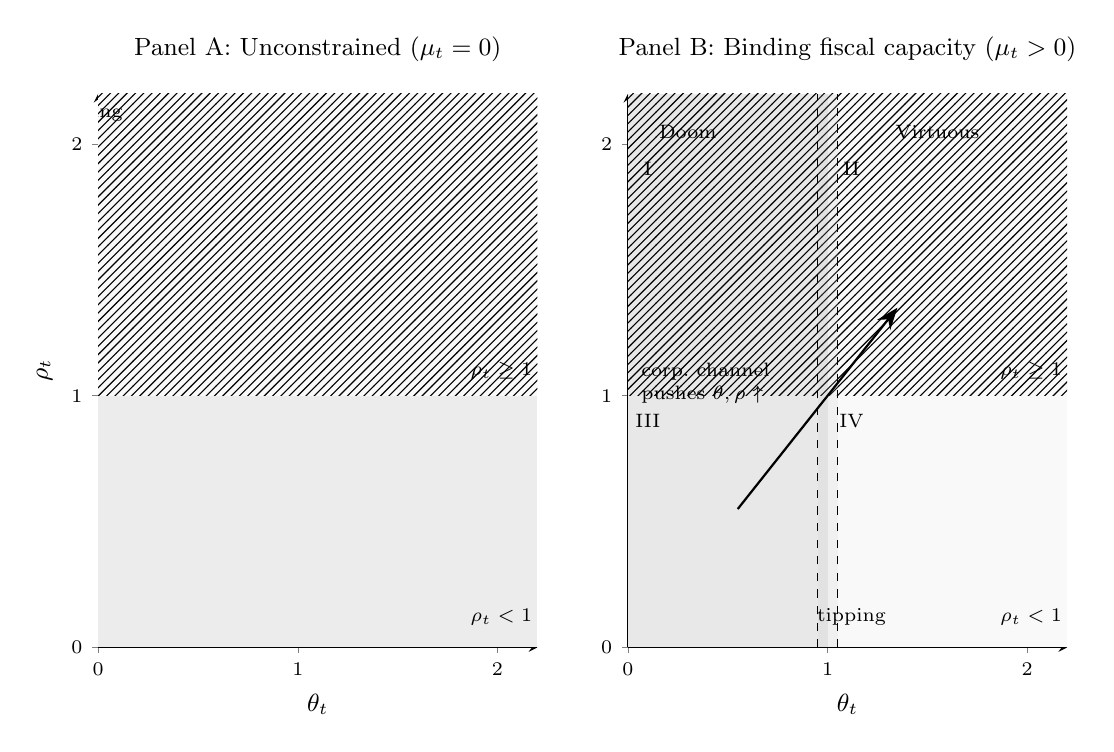
\begin{tikzpicture}
\begin{groupplot}[
    group style={group size=2 by 1, horizontal sep=1.15cm},
    scale only axis,
    width=0.46\linewidth,
    height=0.58\linewidth,
    xmin=0, xmax=2.2,
    ymin=0, ymax=2.2,
    axis lines=left,
    xtick={0,1,2},
    ytick={0,1,2},
    ticklabel style={font=\scriptsize},
    label style={font=\small},
    xlabel={$\theta_t$},
]

%========================
% Panel A: mu=0
%========================
\nextgroupplot[
    title={Panel A: Unconstrained ($\mu_t=0$)},
    title style={font=\small, yshift=2pt},
    ylabel={$\rho_t$},
]

% reference vertical line theta=1 (thin dashed)
\addplot[gray!70, thin, dashed] coordinates {(1,0) (1,2.2)};

% horizontal threshold rho=1 (thick)
\addplot[black, thick] coordinates {(0,1) (2.2,1)};

% shade rho regions
\path[fill=gray!15] (axis cs:0,0) rectangle (axis cs:2.2,1);
\path[fill=gray!05, postaction={pattern=north east lines}] (axis cs:0,1) rectangle (axis cs:2.2,2.2);

% minimal labels
\node[font=\scriptsize] at (axis cs:2.02,1.10) {$\rho_t\ge 1$};
\node[font=\scriptsize] at (axis cs:2.02,0.12) {$\rho_t<1$};
\node[font=\scriptsize, align=left, text width=3.0cm] at (axis cs:0.08,2.08)
{self-financing\\on impact};

%========================
% Panel B: mu>0
%========================
\nextgroupplot[
    title={Panel B: Binding fiscal capacity ($\mu_t>0$)},
    title style={font=\small, yshift=2pt},
    ylabel={}, % do NOT repeat ylabel on the right panel
]

% main boundaries
\addplot[black, thick] coordinates {(1,0) (1,2.2)};      % theta=1 (Prop 7)
\addplot[black, thick] coordinates {(0,1) (2.2,1)};      % rho=1 (Cor 4)

% doom vs virtuous shading (left vs right)
\path[fill=gray!18] (axis cs:0,0) rectangle (axis cs:1,2.2);     % doom side
\path[fill=gray!05] (axis cs:1,0) rectangle (axis cs:2.2,2.2);   % virtuous side

% overlay self-financing region with pattern (rho>=1)
\path[fill=none, postaction={pattern=north east lines}] (axis cs:0,1) rectangle (axis cs:2.2,2.2);

% tipping band around theta=1 (illustrative)
\path[fill=gray!45, opacity=0.16] (axis cs:0.95,0) rectangle (axis cs:1.05,2.2);
\addplot[black, dashed] coordinates {(0.95,0) (0.95,2.2)};
\addplot[black, dashed] coordinates {(1.05,0) (1.05,2.2)};
\node[font=\scriptsize] at (axis cs:1.12,0.12) {tipping};

% ultra-compact labels (no quadrant phrases)
\node[font=\scriptsize] at (axis cs:0.30,2.05) {Doom};
\node[font=\scriptsize] at (axis cs:1.55,2.05) {Virtuous};
\node[font=\scriptsize] at (axis cs:2.02,1.10) {$\rho_t\ge 1$};
\node[font=\scriptsize] at (axis cs:2.02,0.12) {$\rho_t<1$};

% optional quadrant markers (I--IV) for easy referencing without clutter
\node[font=\scriptsize] at (axis cs:0.10,1.90) {I};
\node[font=\scriptsize] at (axis cs:1.12,1.90) {II};
\node[font=\scriptsize] at (axis cs:0.10,0.90) {III};
\node[font=\scriptsize] at (axis cs:1.12,0.90) {IV};

% arrow: corporate channel / credibility pushes (theta, rho) up
\draw[-{Stealth[length=2.8mm]}, thick] (axis cs:0.55,0.55) -- (axis cs:1.35,1.35);
\node[font=\scriptsize, align=left, text width=2.6cm] at (axis cs:0.58,1.05)
{corp.\ channel\\pushes $\theta,\rho\uparrow$};

\end{groupplot}
\end{tikzpicture}

\caption{Regime map accompanying Proposition~\ref{prop:doom_virtuous_regimes}.
Panel A ($\mu_t=0$) emphasizes the self-financing threshold $\rho_t=1$.
Panel B ($\mu_t>0$) highlights the doom vs.\ virtuous boundary at $\theta_t=1$;
the shaded band around $\theta_t\approx 1$ is illustrative of where tipping/multiplicity is more likely under strong feedback
(Corollary~6). In Panel B, quadrants I--IV follow the standard convention (upper-left, upper-right, lower-left, lower-right).}
\label{fig:regime_map_two_panel_clean}
\end{figure}




Figure~\ref{fig:regime_map_two_panel_clean} summarizes the identification logic in a two-panel regime map.
Panel A ($\mu_t=0$) highlights the role of $\rho_t$ for the contemporaneous fiscal return to adaptation. Panel B ($\mu_t>0$) highlights
the doom versus virtuous boundary at $\theta_t=1$, with a narrow band around $\theta_t\approx 1$ illustrating heightened tipping risk.

\subsubsection{Corporate channel and public--private complementarity}
\label{subsec:corporate_channel_B}

The corporate channel expands the virtuous region through two effects captured by \eqref{eq:rho_theta_def_B}.
First, by reducing aggregate corporate spreads, adaptation releases private resources absorbed by financing frictions, increasing
$\rho_t$ through $\Psi_{\bar s^c}(-\partial \bar s^c_t/\partial G_t)$. Second, improved private financial conditions can feed back into
sovereign risk, strengthening the sovereign spread response $-\partial s^g_t/\partial G_t$ and increasing $\theta_t$.
In the regime map, these effects shift the economy upward and to the right, making self-financing on impact more likely and reducing the
set of states in which fiscal tightness triggers a doom loop.





\setcounter{table}{0}
\setcounter{figure}{0}
\renewcommand{\thetable}{\arabic{table}}
\renewcommand{\thefigure}{\arabic{figure}}
\section{Empirical Evidence}
\label{sec:empirical}

This section provides reduced-form evidence for the model's main mechanism. I first test whether adaptation readiness is associated with lower sovereign spreads. I then construct an empirical measure of spread relief and ask whether it sorts debt dynamics into debt-worsening and debt-improving regions. The evidence is interpreted as mechanism-consistent rather than causal, because the adaptation proxy captures broad readiness rather than directly observed public adaptation outlays.

\subsection{Data, Proxies, and Measurement Units}

The sample is an unbalanced country-year panel covering 1995--2023. The United States is excluded because sovereign spreads are measured relative to the U.S. benchmark. The main spread outcome is $s_{it}$, and debt exposure is debt/GDP, $B_{it}$.

The two climate proxies come from the GDP-adjusted ND-GAIN measures. I denote GDP-adjusted readiness by $G_{it}$ and GDP-adjusted vulnerability-performance by $X_{it}$; both compare a country's observed score with the score predicted by GDP per capita in the same year. I use these adjusted measures to separate relative adaptation performance from the broader level of economic development. Higher values of both proxies indicate better performance: higher readiness relative to GDP for $G_{it}$, and lower vulnerability relative to GDP for $X_{it}$.

All ratio and rate variables are kept in share units, so 0.01 corresponds to one percentage point. The control vector $\mathbf{Z}_{it}$ includes standard macroeconomic, fiscal, external-liquidity, institutional, and terms-of-trade controls. The main specifications include country and year fixed effects. Robust $t$-statistics are reported in parentheses. Table~\ref{tab:summary_stats} reports descriptive statistics.

\begin{table}[H]\centering
\begin{threeparttable}
\caption{Post-Preprocessing Descriptive Statistics}
\label{tab:summary_stats}
\scriptsize
\setlength{\tabcolsep}{2.6pt}
\begin{tabularx}{\textwidth}{llYYYYYY}
\toprule
Block & Variable & $N$ & Mean & SD & Median & Min. & Max. \\
\midrule
$S$ & Sovereign spread & 1,272 & 0.024 & 0.043 & 0.007 & -0.034 & 0.343 \\
$G$ & GDP-adj. readiness performance & 1,798 & 0.058 & 0.089 & 0.048 & -0.326 & 0.303 \\
$B$ & Debt/GDP & 1,712 & 0.586 & 0.342 & 0.522 & 0.039 & 2.610 \\
$X$ & GDP-adj. vulnerability performance & 1,798 & -0.040 & 0.058 & -0.047 & -0.185 & 0.295 \\
$Z_1$ & Real GDP & 1,791 & 0.080 & 0.029 & 0.077 & 0.019 & 0.163 \\
$Z_2$ & Real GDP growth & 1,787 & 0.034 & 0.036 & 0.035 & -0.145 & 0.246 \\
$Z_3$ & CPI inflation & 1,791 & 0.057 & 0.108 & 0.032 & -0.018 & 1.973 \\
$Z_4$ & Overall balance/GDP & 1,697 & -0.004 & 0.034 & -0.005 & -0.300 & 0.234 \\
$Z_5$ & International reserves & 1,753 & 0.055 & 0.128 & 0.018 & 0.000 & 1.527 \\
$Z_6$ & Government effectiveness & 1,550 & 0.006 & 0.009 & 0.007 & -0.013 & 0.025 \\
$Z_7$ & Regulatory quality & 1,550 & 0.006 & 0.008 & 0.007 & -0.013 & 0.023 \\
$Z_8$ & Terms of trade & 1,595 & 1.006 & 0.187 & 0.994 & 0.319 & 2.731 \\
\bottomrule
\end{tabularx}
\begin{tablenotes}[flushleft]\footnotesize
\item Notes: Statistics use the post-preprocessing non-U.S. 1995--2023 panel. Each row is computed on nonmissing observations for the corresponding variable.
\end{tablenotes}
\end{threeparttable}
\end{table}

\subsection{Adaptation and Sovereign Financing Costs}

The baseline spread regression tests the sign prediction in Proposition 2:
\begin{equation}
s_{it}
=
\alpha_i+\tau_t
+\beta_G G_{it}
+\beta_B B_{it}
+\beta_X X_{it}
+\boldsymbol{\Gamma}'\mathbf{Z}_{it}
+u_{it}.
\label{eq:emp_baseline_spread}
\end{equation}
Table~\ref{tab:baseline_spread} reports the baseline fixed-effects estimate. The coefficient on $G_{it}$ is negative and statistically significant: countries with stronger readiness performance face lower sovereign spreads. Debt/GDP enters positively, as in standard sovereign-risk regressions. The evidence is consistent with Proposition~2, subject to the reduced-form interpretation of the proxy.

\begin{table}[H]\centering
\begin{threeparttable}
\caption{Baseline Fixed-Effects Estimates}
\label{tab:baseline_spread}
\scriptsize
\begin{tabularx}{0.78\textwidth}{lY}
\toprule
Dependent variable & 10-year sovereign spread, $s_{it}$ \\
\midrule
$G_{it}$ & -0.046*** \\
  & (-2.804) \\
$B_{it}$ & 0.043*** \\
  & (6.042) \\
$X_{it}$ & -0.087*** \\
  & (-2.626) \\
\midrule
Controls $\mathbf{Z}_{it}$ & Yes \\
Country FE & Yes \\
Year FE & Yes \\
Sample period & 1995--2023 \\
Countries & 60 \\
Observations & 1,120 \\
Adjusted $R^2$ & 0.900 \\
\bottomrule
\end{tabularx}
\begin{tablenotes}[flushleft]\footnotesize
\item Notes: Robust $t$-statistics are reported in parentheses. *** $p<0.01$, ** $p<0.05$, * $p<0.10$.
\end{tablenotes}
\end{threeparttable}
\end{table}

\subsection{Heterogeneous Spread Relief and the Empirical Debt-Improving Index}

The next step asks whether the spread-relief effect of the GDP-adjusted readiness-performance proxy varies with debt exposure and GDP-adjusted vulnerability performance, as suggested by Corollary 1. The full-interaction spread model is
\begin{equation}
s_{it}
=
\alpha_i+\tau_t
+\beta_GG_{it}
+\beta_BB_{it}
+\beta_XX_{it}
+\beta_{GB}(G_{it}\times B_{it})
+\beta_{GX}(G_{it}\times X_{it})
+\boldsymbol{\Gamma}'\mathbf{Z}_{it}
+u_{it}.
\label{eq:emp_full_interaction_spread}
\end{equation}
For the empirical index construction, the expanded full-interaction specification also allows the marginal effect of $G_{it}$ to vary with the control vector:
\begin{equation}
\begin{aligned}
s_{it}
&=
\alpha_i+\tau_t
+\beta_GG_{it}
+\beta_BB_{it}
+\beta_XX_{it} \\
&\quad
+\beta_{GB}(G_{it}\times B_{it})
+\beta_{GX}(G_{it}\times X_{it})
+\boldsymbol{\Pi}'(G_{it}\times\mathbf{Z}_{it})
+\boldsymbol{\Gamma}'\mathbf{Z}_{it}
+u_{it}.
\end{aligned}
\label{eq:emp_full_interaction_spread_gz}
\end{equation}
Here, $G_{it}\times\mathbf{Z}_{it}$ denotes the vector of interactions between $G_{it}$ and each component of $\mathbf{Z}_{it}$. The implied marginal effect of $G_{it}$ in equation~\eqref{eq:emp_full_interaction_spread_gz} is
\begin{equation}
\frac{\partial s_{it}}{\partial G_{it}}
=
\beta_G
+\beta_{GB}B_{it}
+\beta_{GX}X_{it}
+\boldsymbol{\Pi}'\mathbf{Z}_{it}.
\label{eq:emp_marginal_spread}
\end{equation}
The implied marginal spread relief and empirical debt-improving index are
\begin{equation}
\widehat m^{G,F}_{it}
=
-
\frac{\partial \widehat s_{it}}{\partial G_{it}},
\qquad
\widehat\theta^F_{it}
=
B_{it}\widehat m^{G,F}_{it}.
\label{eq:emp_theta}
\end{equation}
The index $\widehat\theta^F_{it}$ should be interpreted as an empirical proxy for debt-improving capacity, not as a structural estimate of the theoretical $\theta_t$.

Table~\ref{tab:heterogeneity_spread} reports the interaction estimates. Spread relief from $G_{it}$ is stronger at higher debt levels, as shown by the negative $G_{it}\times B_{it}$ coefficient. The full-interaction columns also allow relief to vary with vulnerability performance and the control vector. Table~\ref{tab:theta_stats} summarizes the resulting index, $\widehat\theta^F_{it}=B_{it}\widehat m^{G,F}_{it}$. This is a proxy-scaled sorting variable, not a structural estimate of the theoretical threshold $\theta_t=1$.

\begin{table}[H]\centering
\begin{threeparttable}
\caption{Heterogeneous Spread Relief}
\label{tab:heterogeneity_spread}
\scriptsize
\setlength{\tabcolsep}{3.0pt}
\begin{tabularx}{\textwidth}{lYYYY}
\toprule
Dependent variable & \multicolumn{4}{c}{10-year sovereign spread, $s_{it}$} \\
\midrule
$G_{it}$ & 0.053** & -0.046*** & 0.058** & 0.319*** \\
  & (2.116) & (-2.791) & (2.271) & (4.651) \\
$B_{it}$ & 0.062*** & 0.044*** & 0.064*** & 0.070*** \\
  & (6.922) & (6.056) & (6.995) & (7.456) \\
$X_{it}$ & -0.052 & -0.084** & -0.043 & 0.086* \\
  & (-1.562) & (-2.485) & (-1.244) & (1.900) \\
$G_{it}\times B_{it}$ & -0.211*** &  & -0.221*** & -0.266*** \\
  & (-4.795) &  & (-4.892) & (-5.723) \\
$G_{it}\times X_{it}$ &  & 0.121 & 0.268** & 0.339** \\
  &  & (1.196) & (2.302) & (2.255) \\
\midrule
Controls $\mathbf{Z}_{it}$ & Yes & Yes & Yes & Yes \\
$G_{it}\times\mathbf{Z}_{it}$ controls & No & No & No & Yes \\
Country FE & Yes & Yes & Yes & Yes \\
Year FE & Yes & Yes & Yes & Yes \\
Countries & 60 & 60 & 60 & 60 \\
Observations & 1,120 & 1,120 & 1,120 & 1,120 \\
Adjusted $R^2$ & 0.905 & 0.900 & 0.906 & 0.911 \\
\bottomrule
\end{tabularx}
\begin{tablenotes}[flushleft]\footnotesize
\item Notes: Columns 1--4 report debt heterogeneity, GDP-adjusted vulnerability-performance heterogeneity, full interaction, and full interaction with $G_{it}\times\mathbf{Z}_{it}$, respectively. Robust $t$-statistics are reported in parentheses. *** $p<0.01$, ** $p<0.05$, * $p<0.10$.
\end{tablenotes}
\end{threeparttable}
\end{table}

\begin{table}[H]\centering
\begin{threeparttable}
\caption{Empirical Debt-Improving Index Descriptive Statistics}
\label{tab:theta_stats}
\scriptsize
\setlength{\tabcolsep}{3.0pt}
\begin{tabularx}{0.88\textwidth}{lYYYYYY}
\toprule
Variable & $N$ & Mean & SD & Median & Min. & Max. \\
\midrule
$\widehat{\theta}^{F}_{it}$ & 1,120 & 0.062 & 0.151 & 0.020 & -0.094 & 1.285 \\
$\widehat m^{G,F}_{it}$ & 1,120 & 0.056 & 0.106 & 0.044 & -0.184 & 0.562 \\
$\partial \widehat s_{it}/\partial G_{it}$ & 1,120 & -0.056 & 0.106 & -0.044 & -0.562 & 0.184 \\
\bottomrule
\end{tabularx}
\begin{tablenotes}[flushleft]\footnotesize
\item Notes: Statistics are computed on the expanded full-interaction spread-model estimation sample. The marginal relief variable is $\widehat m^{G,F}_{it}= -\partial \widehat s_{it}/\partial G_{it}$, and the empirical debt-improving index is $\widehat\theta^F_{it}=B_{it}\widehat m^{G,F}_{it}$.
\end{tablenotes}
\end{threeparttable}
\end{table}

\subsection{Visualizing Spread Relief and the Empirical Index}

Figure~\ref{fig:spread_relief} plots the implied marginal spread relief, $-\partial \widehat s_{it}/\partial G_{it}$. Panel A varies debt/GDP, and Panel B varies vulnerability performance. The figure shows that the estimated relief increases with debt exposure and is larger for more vulnerable observations.

\begin{figure}[H]\centering
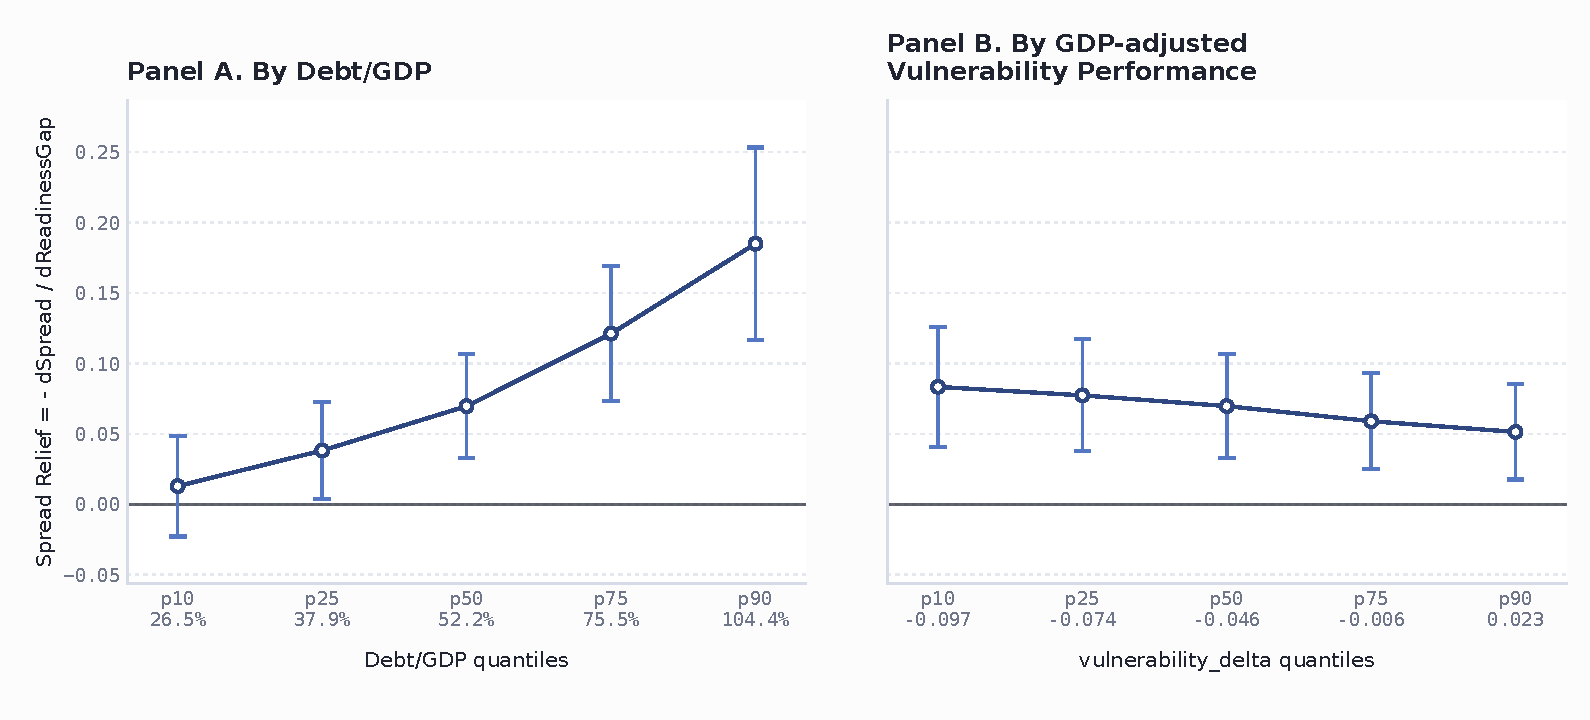
\includegraphics[width=\textwidth]{../best2/result/figure2.pdf}
\caption{Marginal Spread Relief from the Full-Interaction Spread Model}
\label{fig:spread_relief}
\begin{minipage}{0.96\textwidth}
\footnotesize
\textit{Notes:} Panel A fixes $X_{it}$ at its median. Panel B fixes $B_{it}$ at its median. Higher $X_{it}$ indicates lower vulnerability relative to GDP-predicted vulnerability, so the downward slope in Panel B indicates stronger spread relief among more vulnerable observations.
\end{minipage}
\end{figure}

Figure~\ref{fig:theta_distribution} plots the country-year distribution of $\widehat\theta^F_{it}$ and country-level average rankings. The dashed line marks the preferred empirical cutoff selected by the kink specification below. It should not be interpreted as the theoretical threshold $\theta_t=1$.

\begin{figure}[H]\centering
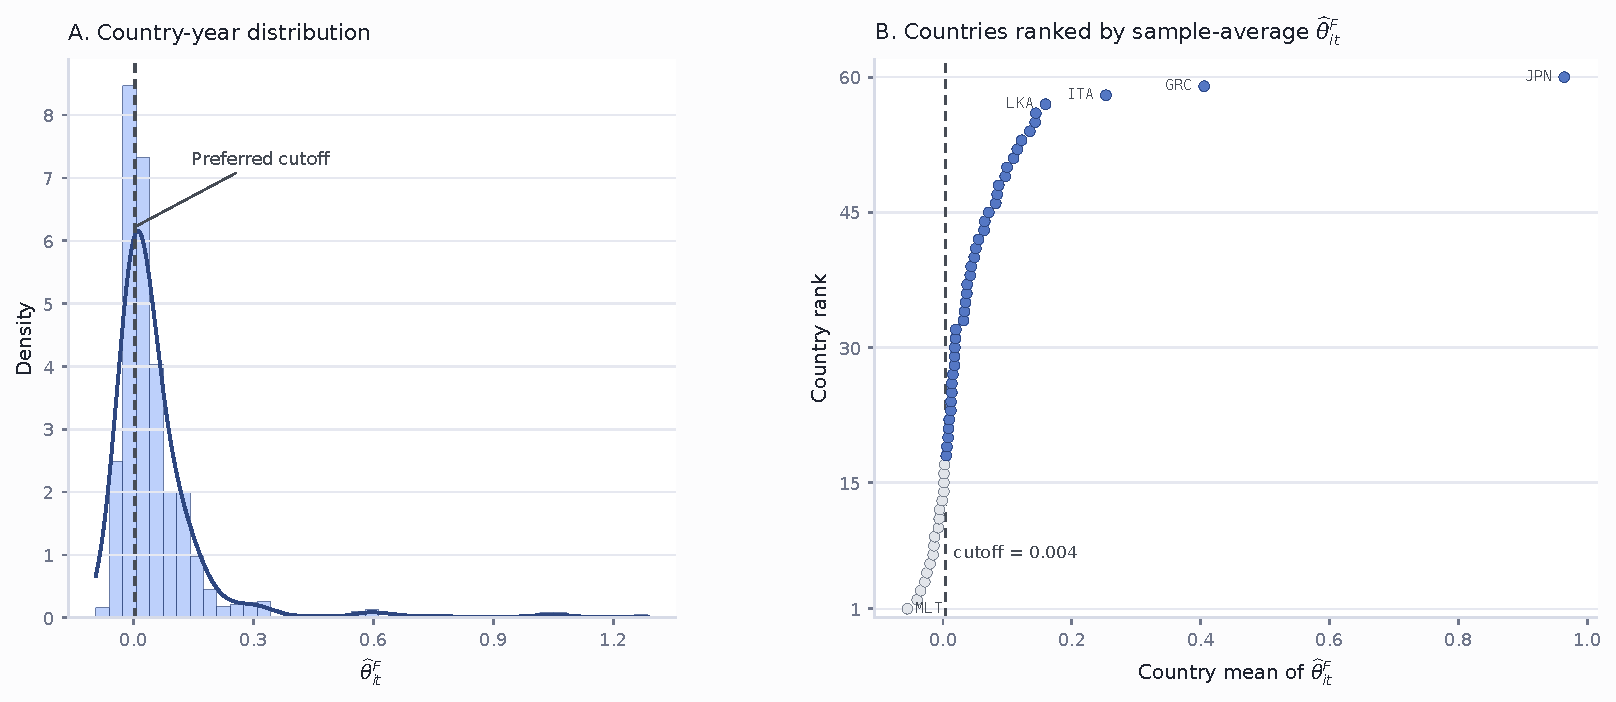
\includegraphics[width=\textwidth]{../best2/result/figure1_theta_distribution_cutoff.pdf}
\caption{Distribution of the Empirical Debt-Improving Index}
\label{fig:theta_distribution}
\begin{minipage}{0.96\textwidth}
\footnotesize
\textit{Notes:} The left panel plots the country-year distribution of $\widehat\theta^F_{it}$. The right panel ranks countries by sample-average $\widehat\theta^F_{it}$. The dashed line marks the preferred empirical cutoff from the without-theta-controls kink specification.
\end{minipage}
\end{figure}

\subsection{Debt Dynamics and the Continuous Theta Interaction}

The next set of tests asks whether the GDP-adjusted readiness-performance proxy is associated with next-period debt changes in a way that varies with the empirical debt-improving index. Define
\begin{equation}
\Delta B_{i,t+1}
=
B_{i,t+1}-B_{it}.
\label{eq:emp_deltaB}
\end{equation}
The baseline debt-change regression is
\begin{equation}
\Delta B_{i,t+1}
=
\alpha_i+\tau_t
+\lambda_0G_{it}
+\boldsymbol{\Gamma}'\mathbf{Z}_{it}
+\varepsilon_{it},
\label{eq:emp_debt_baseline}
\end{equation}
and the continuous theta interaction model is
\begin{equation}
\Delta B_{i,t+1}
=
\alpha_i+\tau_t
+\lambda_0G_{it}
+\lambda_1(G_{it}\times\widehat\theta^F_{it})
+\boldsymbol{\Gamma}'\mathbf{Z}_{it}
+\varepsilon_{it}.
\label{eq:emp_debt_theta}
\end{equation}
Table~\ref{tab:debt_change} reports the continuous theta-interaction test. The coefficient on $G_{it}\times\widehat\theta^F_{it}$ is negative in Column 2, indicating that the debt effect of readiness declines as estimated debt-improving capacity rises. Column 3 adds the theta main effect; the interaction becomes weaker, consistent with interpreting $\widehat\theta^F_{it}$ primarily as a sorting variable.

\begin{table}[H]\centering
\begin{threeparttable}
\caption{Debt-Change Regressions}
\label{tab:debt_change}
\scriptsize
\setlength{\tabcolsep}{3.0pt}
\begin{tabularx}{\textwidth}{lYYY}
\toprule
Dependent variable & \multicolumn{3}{c}{$\Delta B_{i,t+1}=B_{i,t+1}-B_{it}$} \\
\midrule
$G_{it}$ & -0.073 & -0.042 & -0.015 \\
 & (-1.463) & (-0.810) & (-0.302) \\
$G_{it}\times\widehat\theta^F_{it}$ &  & -0.886*** & -0.310 \\
 &  & (-2.707) & (-0.660) \\
$\widehat\theta^F_{it}$ &  &  & -0.141* \\
 &  &  & (-1.898) \\
\midrule
Theta main effect & No & No & Yes \\
Controls $\mathbf{Z}_{it}$ & Yes & Yes & Yes \\
Country FE & Yes & Yes & Yes \\
Year FE & Yes & Yes & Yes \\
Observations & 1,060 & 1,060 & 1,060 \\
Countries & 60 & 60 & 60 \\
Adjusted $R^2$ & 0.425 & 0.433 & 0.441 \\
\bottomrule
\end{tabularx}
\begin{tablenotes}[flushleft]\footnotesize
\item Notes: Columns 1--3 report the baseline model, the continuous theta-interaction model, and the specification with a theta main effect. Controls are included but not reported. Robust $t$-statistics are reported in parentheses. *** $p<0.01$, ** $p<0.05$, * $p<0.10$.
\end{tablenotes}
\end{threeparttable}
\end{table}

\subsection{Grouped Debt-Change Heterogeneity}

Table~\ref{tab:grouped_debt_change} reports quintile regressions. Sorting by the composite index $\widehat\theta^F_{it}$ gives the clearest pattern: the coefficient on $G_{it}$ is positive in the lowest group and negative in the highest groups. Debt/GDP alone produces a weaker ordering, while marginal relief alone is closer but lacks the debt-exposure component of the model.

\begin{table}[H]\centering
\caption{Grouped Debt-Change Heterogeneity Regressions}
\label{tab:grouped_debt_change}
\begin{threeparttable}
\scriptsize
\setlength{\tabcolsep}{3.0pt}
\renewcommand{\arraystretch}{1.10}
\textbf{Panel A. Full-theta groups}\\[0.45em]
\begin{tabularx}{\textwidth}{lYYYYY}
\toprule
Dependent variable & \multicolumn{5}{c}{$B_{i,t+1}-B_{it}$} \\
\cmidrule(lr){2-6}
Group & 0--20\% & 20--40\% & 40--60\% & 60--80\% & 80--100\% \\
\midrule
$G_{it}$ & 0.243* & 0.057 & -0.152 & -0.249* & -0.372** \\
 & (1.727) & (0.866) & (-1.550) & (-1.770) & (-2.077) \\
\midrule
Controls $\mathbf{Z}_{it}$ & Yes & Yes & Yes & Yes & Yes \\
Country FE & Yes & Yes & Yes & Yes & Yes \\
Year FE & Yes & Yes & Yes & Yes & Yes \\
Observations & 212 & 212 & 212 & 212 & 212 \\
Countries & 25 & 33 & 35 & 37 & 22 \\
Adjusted $R^2$ & 0.604 & 0.669 & 0.499 & 0.366 & 0.522 \\
\bottomrule
\end{tabularx}

\vspace{0.75em}
\textbf{Panel B. Debt-ratio groups}\\[0.45em]
\begin{tabularx}{\textwidth}{lYYYYY}
\toprule
Dependent variable & \multicolumn{5}{c}{$B_{i,t+1}-B_{it}$} \\
\cmidrule(lr){2-6}
Group & 0--20\% & 20--40\% & 40--60\% & 60--80\% & 80--100\% \\
\midrule
$G_{it}$ & 0.060 & -0.116 & -0.067 & 0.038 & -0.363 \\
 & (0.861) & (-1.336) & (-1.021) & (0.291) & (-1.317) \\
\midrule
Controls $\mathbf{Z}_{it}$ & Yes & Yes & Yes & Yes & Yes \\
Country FE & Yes & Yes & Yes & Yes & Yes \\
Year FE & Yes & Yes & Yes & Yes & Yes \\
Observations & 212 & 212 & 212 & 212 & 212 \\
Countries & 28 & 35 & 41 & 32 & 22 \\
Adjusted $R^2$ & 0.466 & 0.483 & 0.700 & 0.394 & 0.625 \\
\bottomrule
\end{tabularx}

\vspace{0.75em}
\textbf{Panel C. Marginal-relief groups}\\[0.45em]
\begin{tabularx}{\textwidth}{lYYYYY}
\toprule
Dependent variable & \multicolumn{5}{c}{$B_{i,t+1}-B_{it}$} \\
\cmidrule(lr){2-6}
Group & 0--20\% & 20--40\% & 40--60\% & 60--80\% & 80--100\% \\
\midrule
$G_{it}$ & 0.325** & 0.097 & -0.041 & -0.134 & -0.512*** \\
 & (2.244) & (0.732) & (-0.426) & (-1.350) & (-3.273) \\
\midrule
Controls $\mathbf{Z}_{it}$ & Yes & Yes & Yes & Yes & Yes \\
Country FE & Yes & Yes & Yes & Yes & Yes \\
Year FE & Yes & Yes & Yes & Yes & Yes \\
Observations & 212 & 212 & 212 & 212 & 212 \\
Countries & 25 & 36 & 36 & 34 & 24 \\
Adjusted $R^2$ & 0.603 & 0.568 & 0.518 & 0.606 & 0.493 \\
\bottomrule
\end{tabularx}
\begin{tablenotes}[flushleft]\footnotesize
\item Notes: Each column estimates the next-period change in debt/GDP on current GDP-adjusted readiness performance, $G_{it}$, within the indicated subgroup. Macro control coefficients and subgroup cutoff values are omitted for compactness. Robust $t$-statistics are reported in parentheses. *** $p<0.01$, ** $p<0.05$, * $p<0.10$.
\end{tablenotes}
\end{threeparttable}
\end{table}

\subsection{Single-Crossing Kink Test}

The single-crossing specification provides the closest empirical analogue to Corollary 4 and its mirror image. It directly tests whether the marginal effect of the adaptation-readiness proxy on next-period debt changes switches sign around an empirical cutoff. This specification is not a standard panel threshold model. It is designed to estimate whether the marginal debt effect of $G_{it}$ crosses zero as a function of $\widehat\theta^F_{it}$.

For a candidate cutoff $c$, the estimated specification is
\begin{equation}
\Delta B_{i,t+1}
=
\alpha_i+\tau_t
+aG_{it}(c-\widehat\theta^F_{it})_+
+bG_{it}(\widehat\theta^F_{it}-c)_+
+\boldsymbol{\Gamma}'\mathbf{Z}_{it}
+\varepsilon_{it}.
\label{eq:emp_kink}
\end{equation}
The implied marginal effect is
\begin{equation}
m(\theta;c)
=
a(c-\theta)_+
+
b(\theta-c)_+.
\label{eq:emp_kink_marginal}
\end{equation}
The theoretical sign pattern is
\[
a>0,
\qquad
b<0.
\]

Table~\ref{tab:kink_model} selects an empirical cutoff of $c=0.004123$. The estimated marginal effect is positive below the cutoff and negative above it, matching the debt-worsening/debt-improving sign pattern. The cutoff is a proxy-scaled empirical boundary rather than the literal theoretical threshold $\theta_t=1$.

\begin{table}[H]\centering
\begin{threeparttable}
\caption{Single-Crossing Kink Marginal-Effect Model}
\label{tab:kink_model}
\scriptsize
\setlength{\tabcolsep}{3.0pt}
\begin{tabularx}{0.78\textwidth}{lY}
\toprule
Dependent variable & $B_{i,t+1}-B_{it}$ \\
\midrule
$G_{it}(c-\widehat\theta^F_{it})_+$ & 3.380*** \\
 & (2.592) \\
$G_{it}(\widehat\theta^F_{it}-c)_+$ & -0.804** \\
 & (-2.464) \\
\midrule
Cutoff $c$ & 0.004 \\
RSS & 1.951 \\
Share below cutoff & 0.350 \\
Selection rule & RSS minimum; sign-consistent \\
Controls $\mathbf{Z}_{it}$ & Yes \\
Country FE & Yes \\
Year FE & Yes \\
Observations & 1,060 \\
Adjusted $R^2$ & 0.435 \\
\bottomrule
\end{tabularx}
\begin{tablenotes}[flushleft]\footnotesize
\item Notes: The exact RSS-selected cutoff is $c=0.0041231435658208$. The model includes country and year fixed effects and $\mathbf{Z}_{it}$ controls, but does not include direct theta controls. Robust $t$-statistics are reported in parentheses. *** $p<0.01$, ** $p<0.05$.
\end{tablenotes}
\end{threeparttable}
\end{table}

Figure~\ref{fig:kink_marginal_effect} plots the continuous marginal-effect curve implied by equation~\eqref{eq:emp_kink_marginal}. The left side of the cutoff corresponds to the debt-worsening region, while the right side corresponds to the debt-improving region.

\begin{figure}[H]\centering
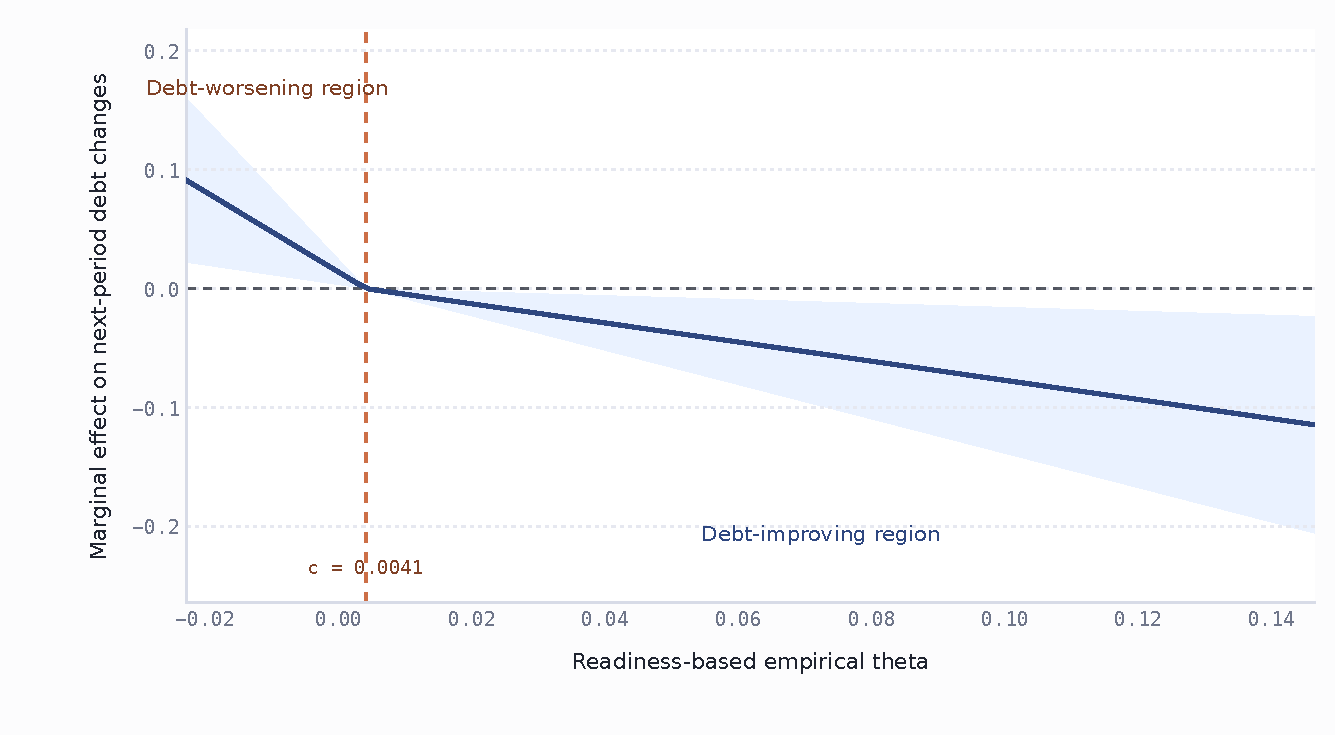
\includegraphics[width=0.92\textwidth]{../best2/result/figure3_kink_marginal_effect_notheta_continuous.pdf}
\caption{Continuous Kink Marginal Effect without Theta Controls}
\label{fig:kink_marginal_effect}
\begin{minipage}{0.92\textwidth}
\footnotesize
\textit{Notes:} The figure plots $m(\theta;c)=a(c-\theta)_+ + b(\theta-c)_+$ from the single-crossing kink model without theta controls. Positive values imply that readiness improvements are associated with higher next-period debt changes; negative values imply lower next-period debt changes. The vertical dashed line marks the empirical cutoff $c$.
\end{minipage}
\end{figure}

\subsection{Country Screens Around the Preferred Cutoff}

Finally, Table~\ref{tab:country_screens} reports an illustrative country-level screen based on the preferred cutoff. The exercise is descriptive and should be read as a diagnostic use of the index, not as a structural country ranking.

Future work can use this screen to choose representative case countries. Following the budget-document approach in Duffy's \textit{Climate Change, Adaptation, and Sovereign Risk}, we can use public budget files and spending reports to identify actual adaptation expenditures, providing a direct benchmark for the readiness proxy and the debt-improving index.

\begin{table}[H]\centering
\begin{threeparttable}
\caption{Country Screens Around the Preferred Cutoff}
\label{tab:country_screens}
\scriptsize
\setlength{\tabcolsep}{3.0pt}
\textbf{Panel A. Low debt, theta always above the cutoff, and top-quartile marginal relief}\\[0.45em]
\begin{tabularx}{\textwidth}{llYYYYY}
\toprule
Country & ISO3 & Sample period & Years & Mean debt/GDP & Mean theta & Mean $\widehat m^{G,F}$ \\
\midrule
Vietnam & VNM & 2007--2023 & 17 & 39.50\% & 0.065 & 0.164 \\
Indonesia & IDN & 2003--2023 & 21 & 33.72\% & 0.055 & 0.156 \\
Colombia & COL & 2002--2023 & 21 & 45.82\% & 0.064 & 0.134 \\
\bottomrule
\end{tabularx}

\vspace{0.75em}
\textbf{Panel B. High debt, theta always below the cutoff, and bottom-quartile marginal relief}\\[0.45em]
\begin{tabularx}{\textwidth}{llYYYYY}
\toprule
Country & ISO3 & Sample period & Years & Mean debt/GDP & Mean theta & Mean $\widehat m^{G,F}$ \\
\midrule
Malta & MLT & 2010--2023 & 14 & 53.91\% & -0.055 & -0.107 \\
\bottomrule
\end{tabularx}
\begin{tablenotes}[flushleft]\footnotesize
\item Notes: The preferred cutoff is $c=0.004123$. Screening thresholds use country-level means: the mean-debt median is 53.06 percent, the bottom quartile of mean $\widehat m^{G,F}_{it}$ is 0.003, and the top quartile is 0.112. The always-above and always-below conditions are evaluated year by year.
\end{tablenotes}
\end{threeparttable}
\end{table}

\subsection{Summary and Online Appendix Roadmap}

The empirical section delivers three reduced-form patterns. First, GDP-adjusted readiness is negatively associated with sovereign spreads. Second, the implied spread relief is stronger when debt exposure is high and when countries are more vulnerable relative to their GDP-predicted benchmark. Third, the debt-dynamics results are state dependent: readiness is associated with higher next-period debt changes in low-\(\widehat\theta^F_{it}\) regions and lower debt changes in high-\(\widehat\theta^F_{it}\) regions. These findings are consistent with the paper's central mechanism.

The online appendix reports supporting exercises. Appendix~B varies the debt-dynamics specifications and shows that the without-theta-controls kink model gives the clearest single-crossing pattern. Appendix~C repeats the analysis using level ND-GAIN readiness and vulnerability measures. The main readiness and debt-interaction results remain stable, while vulnerability heterogeneity is more proxy-sensitive.



\clearpage
\bibliographystyle{apalike}  % 或 plainnat / abbrvnat，按期刊要求换
\bibliography{ref}          % 对应 ref.bib（不要写 .bib 后缀）





\clearpage
\appendix
\setcounter{equation}{0}
\renewcommand{\theequation}{A.\arabic{equation}}
\setcounter{figure}{0}
\renewcommand{\thefigure}{A.\arabic{figure}}
\section{Proofs}

\subsection{Proof of Proposition~\ref{prop:doom_virtuous_regimes}: Doom vs.\ virtuous loop under a fiscal-capacity constraint}

Consider the government's constrained one-period problem at date $t$:
\begin{equation}
  V^c(S_t)
  =
  \max_{G_t\ge 0}
  \Big\{
    W_t(S_t,G_t)
    + \beta\,\mathbb{E}_t\big[V^c(S_{t+1})\big]
    + \mu_t\big(\overline B(\Xi_t)-B_{t+1}\big)
  \Big\},
  \label{eq:app_constrained_problem}
\end{equation}
where $\mu_t\ge 0$ is the multiplier on the fiscal-capacity constraint \eqref{eq:debt_limit_B}, together with the complementarity
conditions
\begin{equation}
  \mu_t\ge 0,
  \qquad
  \overline B(\Xi_t)-B_{t+1}\ge 0,
  \qquad
  \mu_t\big(\overline B(\Xi_t)-B_{t+1}\big)=0.
  \label{eq:app_complementarity}
\end{equation}

For an interior choice of $G_t$, the first-order condition is
\begin{equation}
  \frac{\partial W_t}{\partial G_t}
  + \beta\,\mathbb{E}_t\!\left[
    V_X^c(S_{t+1})\frac{\partial X_{t+1}}{\partial G_t}
    +V_B^c(S_{t+1})\frac{\partial B_{t+1}}{\partial G_t}
    +V_{\Xi}^c(S_{t+1})\frac{\partial \Xi_{t+1}}{\partial G_t}
  \right]
  - \mu_t\frac{\partial B_{t+1}}{\partial G_t}
  =0.
  \label{eq:app_constrained_foc}
\end{equation}
Relative to the unconstrained first-order condition \eqref{eq:FOC_general_B}, the binding fiscal-capacity constraint adds the wedge
$-\mu_t(\partial B_{t+1}/\partial G_t)$.

Using the debt law of motion in \eqref{eq:dBnext_dG_B} and the definition of $\theta_t$ in \eqref{eq:rho_theta_def_B},
\begin{equation}
  \frac{\partial B_{t+1}}{\partial G_t}
  =
  1 + B_t\frac{\partial s_t^g}{\partial G_t}
  =
  1-\theta_t.
  \label{eq:app_dB_dG_theta}
\end{equation}
Hence \eqref{eq:app_constrained_foc} can be written as
\begin{equation}
  H(G_t,\mu_t;S_t)
  \equiv
  \mathcal{F}(G_t;S_t) - \mu_t\big(1-\theta_t\big)=0,
  \label{eq:app_reduced_foc}
\end{equation}
where
\begin{equation}
  \mathcal{F}(G_t;S_t)
  \equiv
  \frac{\partial W_t}{\partial G_t}
  + \beta\,\mathbb{E}_t\!\left[
    V_X^c(S_{t+1})\frac{\partial X_{t+1}}{\partial G_t}
    +V_B^c(S_{t+1})\frac{\partial B_{t+1}}{\partial G_t}
    +V_{\Xi}^c(S_{t+1})\frac{\partial \Xi_{t+1}}{\partial G_t}
  \right],
  \label{eq:app_F_def}
\end{equation}
and
\begin{equation}
  \theta(G_t;S_t) \equiv B_t\Big(-\frac{\partial s_t^g}{\partial G_t}\Big).
  \label{eq:app_theta_function}
\end{equation}

Assume the strengthened local second-order/regularity condition
\begin{equation}
  H_G(G_t^*,\mu_t;S_t) <0,
  \label{eq:app_soc}
\end{equation}
 Applying the implicit function theorem to \eqref{eq:app_reduced_foc} yields
\begin{equation}
  \frac{\partial G_t^*}{\partial \mu_t}
  =
  -\frac{H_{\mu}(G_t^*,\mu_t;S_t)}{H_G(G_t^*,\mu_t;S_t)}
  =
  \frac{1-\theta_t}{H_G(G_t^*,\mu_t;S_t)},
  \label{eq:app_dG_dmu}
\end{equation}
where $\theta_t\equiv \theta(G_t^*;S_t)$ is evaluated at the optimum. Because the denominator is negative by \eqref{eq:app_soc},
the sign of $\partial G_t^*/\partial \mu_t$ is the opposite of the sign of $1-\theta_t$. 

This proves Proposition~\ref{prop:doom_virtuous_regimes}. \hfill $\square$

\subsection{Proof of Corollary~\ref{cor:tipping_B}: Tipping and local multiplicity}
The local equilibrium choice of adaptation solves the fixed-point problem
\begin{equation}
  G_t
  =
  \mathcal{T}(G_t;S_t)
  \equiv
  \mathcal{G}\!\left(\mathcal{M}\big( B_{t+1}-\overline B(\Xi_t)\big);S_t\right).
  \label{eq:app_fixed_point}
\end{equation}

Differentiating \eqref{eq:app_fixed_point} with respect to $G_t$ and applying the chain rule gives, at a local fixed point $G_t^*$,
\begin{equation}
  \mathcal{T}_G(G_t^*;S_t)
  =
  \frac{\partial \mathcal{G}(\mu_t;S_t)}{\partial \mu_t}
  \cdot
  \mathcal{M}'\!(\cdot)
  \cdot
  \frac{\partial B_{t+1}}{\partial G_t}.
  \label{eq:app_Tprime_step1}
\end{equation}
Using \eqref{eq:dBnext_dG_B},
\begin{equation}
  \frac{\partial B_{t+1}}{\partial G_t}
  =
  1+B_t\frac{\partial s_t^g}{\partial G_t},
  \label{eq:app_Tprime_step2}
\end{equation}
so
\begin{equation}
  \big|\mathcal{T}_G(G_t^*;S_t)\big|
  =
  \big|\partial \mathcal{G}(\mu_t;S_t)/\partial \mu_t\big|
  \big|\mathcal{M}'(\cdot)\big|
  \big|1+B_t(\partial s_t^g/\partial G_t)\big|.
  \label{eq:app_Tprime_final}
\end{equation}
Therefore condition \eqref{eq:tipping_condition_B} is exactly the statement that
\begin{equation}
  \big|\mathcal{T}_G(G_t^*;S_t)\big|>1.
  \label{eq:app_noncontraction}
\end{equation}
oh'g

This proves Corollary~\ref{cor:tipping_B}. \hfill $\square$












\clearpage
\setcounter{table}{0}
\renewcommand{\thetable}{B.\arabic{table}}
\setcounter{figure}{0}
\renewcommand{\thefigure}{B.\arabic{figure}}
\setcounter{equation}{0}
\renewcommand{\theequation}{B.\arabic{equation}}

\section{Additional Empirical Results}
\label{appendixB}

This appendix reports control-set variants for the debt-change and single-crossing kink specifications. The main text treats the without-theta-controls kink model with $\mathbf{Z}_{it}$ controls as the preferred specification. The no-theta-controls kink specification displays the clearest single-crossing pattern. Specifications with direct theta controls preserve the positive low-theta effect but attenuate the high-theta debt-improving effect, suggesting that the evidence is strongest when $\widehat\theta^F_{it}$ is used as the sorting index rather than absorbed directly as an additional control.

\begin{table}[H]\centering
\caption{Debt-Change Model Control-Set Variants}
\label{tab:app_debt_change_control_variants}
\begin{threeparttable}
\scriptsize
\setlength{\tabcolsep}{3.0pt}
\renewcommand{\arraystretch}{1.02}
\textbf{Panel A. Baseline debt-change model}\\[0.45em]
\begin{tabularx}{\textwidth}{lYYY}
\toprule
Dependent variable & \multicolumn{3}{c}{$B_{i,t+1}-B_{it}$} \\
Control set & $\mathbf{Z}+B+X$ & $B+X$ & None \\
\midrule
$G_{it}$ & -0.024 & -0.069 & -0.030 \\
 & (-0.569) & (-1.513) & (-0.577) \\
$B_{it}$ & -0.093*** & -0.098*** &  \\
 & (-3.839) & (-4.607) &  \\
$X_{it}$ & -0.143 & -0.492*** &  \\
 & (-1.241) & (-4.306) &  \\
\midrule
Controls $\mathbf{Z}_{it}$ & Yes & No & No \\
Observations & 1,060 & 1,060 & 1,060 \\
Adjusted $R^2$ & 0.449 & 0.372 & 0.327 \\
\bottomrule
\end{tabularx}

\vspace{0.35em}
\textbf{Panel B. Continuous theta interaction model}\\[0.45em]
\begin{tabularx}{\textwidth}{lYYY}
\toprule
Dependent variable & \multicolumn{3}{c}{$B_{i,t+1}-B_{it}$} \\
Control set & $\mathbf{Z}+B+X$ & $B+X$ & None \\
\midrule
$G_{it}$ & -0.016 & -0.056 & 0.010 \\
 & (-0.370) & (-1.166) & (0.182) \\
$G_{it}\times\widehat{\theta}^{F}_{it}$ & -0.250 & -0.432 & -1.236*** \\
 & (-0.576) & (-1.009) & (-3.504) \\
$B_{it}$ & -0.086*** & -0.087*** &  \\
 & (-2.675) & (-3.183) &  \\
$X_{it}$ & -0.118 & -0.457*** &  \\
 & (-0.974) & (-3.981) &  \\
\midrule
Controls $\mathbf{Z}_{it}$ & Yes & No & No \\
Observations & 1,060 & 1,060 & 1,060 \\
Adjusted $R^2$ & 0.449 & 0.373 & 0.346 \\
\bottomrule
\end{tabularx}

\vspace{0.35em}
\textbf{Panel C. Full-theta dynamics model}\\[0.45em]
\begin{tabularx}{\textwidth}{lYYY}
\toprule
Dependent variable & \multicolumn{3}{c}{$B_{i,t+1}-B_{it}$} \\
Control set & $\mathbf{Z}+B+X$ & $B+X$ & None \\
\midrule
$G_{it}$ & -0.021 & -0.077 & 0.038 \\
 & (-0.473) & (-1.615) & (0.728) \\
$G_{it}\times\widehat{\theta}^{F}_{it}$ & -0.133 & 0.062 & -0.302 \\
 & (-0.267) & (0.138) & (-0.674) \\
$\widehat{\theta}^{F}_{it}$ & -0.044 & -0.188*** & -0.194*** \\
 & (-0.584) & (-2.727) & (-3.320) \\
$B_{it}$ & -0.076** & -0.035 &  \\
 & (-2.369) & (-1.130) &  \\
$X_{it}$ & -0.146 & -0.538*** &  \\
 & (-1.088) & (-4.311) &  \\
\midrule
Controls $\mathbf{Z}_{it}$ & Yes & No & No \\
Observations & 1,060 & 1,060 & 1,060 \\
Adjusted $R^2$ & 0.449 & 0.383 & 0.367 \\
\bottomrule
\end{tabularx}
\begin{tablenotes}[flushleft]\footnotesize
\item Notes: Each specification includes country and year fixed effects. Robust $t$-statistics are reported in parentheses. *** $p<0.01$, ** $p<0.05$.
\end{tablenotes}
\end{threeparttable}
\end{table}

For the $\mathbf{Z}_{it}+B_{it}+X_{it}$ version reported in Table~\ref{tab:app_kink_notheta_controls}, the without-theta-controls kink specification is
\begin{equation}
\begin{aligned}
\Delta B_{i,t+1}
&=
\alpha_i+\tau_t
+aG_{it}(c-\widehat\theta^F_{it})_+
+bG_{it}(\widehat\theta^F_{it}-c)_+ \\
&\quad
+\delta_B B_{it}
+\delta_X X_{it}
+\boldsymbol{\Gamma}'\mathbf{Z}_{it}
+\varepsilon_{it}.
\end{aligned}
\label{eq:app_kink_notheta_zbx}
\end{equation}

\begin{table}[H]\centering
\caption{Single-Crossing Kink without Theta Controls: Control-Set Variants}
\label{tab:app_kink_notheta_controls}
\begin{threeparttable}
\scriptsize
\setlength{\tabcolsep}{3.0pt}
\begin{tabularx}{0.92\textwidth}{lYYY}
\toprule
Dependent variable & \multicolumn{3}{c}{$B_{i,t+1}-B_{it}$} \\
Control set & $\mathbf{Z}+B+X$ & $B+X$ & None \\
\midrule
$G_{it}(c-\widehat\theta^F_{it})_+$ & 3.402** & 3.583 & 4.343** \\
$p(a>0)$ & 0.010 & 0.052 & 0.005 \\
$G_{it}(\widehat\theta^F_{it}-c)_+$ & -0.154 & -0.345 & -1.061*** \\
$p(b<0)$ & 0.360 & 0.205 & 0.001 \\
\midrule
RSS cutoff & 0.004 & -0.003 & 0.006 \\
Sign-consistent & Yes & Yes & Yes \\
Country FE & Yes & Yes & Yes \\
Year FE & Yes & Yes & Yes \\
Observations & 1,060 & 1,060 & 1,060 \\
Adjusted $R^2$ & 0.452 & 0.375 & 0.351 \\
\bottomrule
\end{tabularx}
\begin{tablenotes}[flushleft]\footnotesize
\item Notes: These variants keep the main without-theta-controls kink structure but vary the additional controls. The preferred main-text cutoff remains the $\mathbf{Z}_{it}$-controls specification. Reported $p$-values are one-sided tests for the sign restriction. *** $p<0.01$, ** $p<0.05$.
\end{tablenotes}
\end{threeparttable}
\end{table}

For the $\mathbf{Z}_{it}+B_{it}+X_{it}$ version corresponding to Table~\ref{tab:app_kink_withtheta_main}, the kink specification with direct theta controls is
\begin{equation}
\begin{aligned}
\Delta B_{i,t+1}
&=
\alpha_i+\tau_t
+aG_{it}(c-\widehat\theta^F_{it})_+
+bG_{it}(\widehat\theta^F_{it}-c)_+ \\
&\quad
+\rho_1\widehat\theta^F_{it}
+\rho_2(\widehat\theta^F_{it}-c)_+
+\delta_B B_{it}
+\delta_X X_{it}
+\boldsymbol{\Gamma}'\mathbf{Z}_{it}
+\varepsilon_{it}.
\end{aligned}
\label{eq:app_kink_withtheta_zbx_main}
\end{equation}

\begin{table}[H]\centering
\begin{threeparttable}
\caption{Single-Crossing Kink with Theta Controls}
\label{tab:app_kink_withtheta_main}
\scriptsize
\setlength{\tabcolsep}{3.0pt}
\begin{tabularx}{0.78\textwidth}{lY}
\toprule
Dependent variable & $B_{i,t+1}-B_{it}$ \\
\midrule
$G_{it}(c-\widehat\theta^F_{it})_+$ & 3.560*** \\
 & (3.163) \\
$G_{it}(\widehat\theta^F_{it}-c)_+$ & -0.113 \\
 & (-0.233) \\
\midrule
Direct theta controls & Yes \\
Cutoff $c$ & 0.004 \\
RSS & 1.889 \\
Share below cutoff & 0.350 \\
Selection rule & RSS minimum; sign-consistent \\
Controls $\mathbf{Z}_{it}$ & Yes \\
Country FE & Yes \\
Year FE & Yes \\
Observations & 1,060 \\
Adjusted $R^2$ & 0.452 \\
\bottomrule
\end{tabularx}
\begin{tablenotes}[flushleft]\footnotesize
\item Notes: This appendix version includes $\widehat{\theta}^{F}_{it}$ and $(\widehat{\theta}^{F}_{it}-c)_+$ as direct controls. The low-theta coefficient remains positive and significant, but the high-theta debt-improving coefficient is much weaker. Robust $t$-statistics are reported in parentheses. *** $p<0.01$.
\end{tablenotes}
\end{threeparttable}
\end{table}

For the $\mathbf{Z}_{it}+B_{it}+X_{it}$ column reported in Table~\ref{tab:app_kink_withtheta_controls}, the estimated with-theta-controls variant uses the same control-augmented kink equation:
\begin{equation}
\begin{aligned}
\Delta B_{i,t+1}
&=
\alpha_i+\tau_t
+aG_{it}(c-\widehat\theta^F_{it})_+
+bG_{it}(\widehat\theta^F_{it}-c)_+ \\
&\quad
+\rho_1\widehat\theta^F_{it}
+\rho_2(\widehat\theta^F_{it}-c)_+
+\delta_B B_{it}
+\delta_X X_{it}
+\boldsymbol{\Gamma}'\mathbf{Z}_{it}
+\varepsilon_{it}.
\end{aligned}
\label{eq:app_kink_withtheta_zbx_variants}
\end{equation}

\begin{table}[H]\centering
\caption{Single-Crossing Kink with Theta Controls: Control-Set Variants}
\label{tab:app_kink_withtheta_controls}
\begin{threeparttable}
\scriptsize
\setlength{\tabcolsep}{3.0pt}
\begin{tabularx}{0.92\textwidth}{lYYY}
\toprule
Dependent variable & \multicolumn{3}{c}{$B_{i,t+1}-B_{it}$} \\
Control set & $\mathbf{Z}+B+X$ & $B+X$ & None \\
\midrule
$G_{it}(c-\widehat\theta^F_{it})_+$ & 3.303* & 2.576 & 5.873*** \\
$p(a>0)$ & 0.044 & 0.075 & 0.000 \\
$G_{it}(\widehat\theta^F_{it}-c)_+$ & -0.101 & 0.018 & -0.020 \\
$p(b<0)$ & 0.416 & 0.516 & 0.482 \\
\midrule
RSS cutoff & -0.012 & -0.004 & -0.004 \\
Sign-consistent & Yes & No & Yes \\
Direct theta controls & Yes & Yes & Yes \\
Country FE & Yes & Yes & Yes \\
Year FE & Yes & Yes & Yes \\
Observations & 1,060 & 1,060 & 1,060 \\
Adjusted $R^2$ & 0.456 & 0.401 & 0.387 \\
\bottomrule
\end{tabularx}
\begin{tablenotes}[flushleft]\footnotesize
\item Notes: These variants keep direct theta controls and vary the additional controls across $\mathbf{Z}_{it}+B_{it}+X_{it}$, $B_{it}+X_{it}$, and no controls. Reported $p$-values are one-sided tests for the sign restriction. *** $p<0.01$, * $p<0.10$.
\end{tablenotes}
\end{threeparttable}
\end{table}

\clearpage
\setcounter{table}{0}
\renewcommand{\thetable}{C.\arabic{table}}
\setcounter{figure}{0}
\renewcommand{\thefigure}{C.\arabic{figure}}
\setcounter{equation}{0}
\renewcommand{\theequation}{C.\arabic{equation}}

\section{Alternative Empirical Results Using Level Readiness and Vulnerability}
\label{appendixC}

This appendix repeats the empirical exercise in Section~\ref{sec:empirical} using level ND-GAIN readiness and vulnerability measures instead of the GDP-adjusted residual-performance measures used in the main specification. The purpose is to assess whether the reduced-form spread, debt-dynamics, and single-crossing patterns are sensitive to this alternative proxy construction. The empirical workflow, sample restrictions, fixed effects, and standard-error convention are otherwise unchanged.

\subsection{Data, Proxies, and Measurement Units}

The sample is the same unbalanced non-U.S. country-year panel covering 1995--2023. The dependent variable in the spread regressions is the sovereign spread, $s_{it}$. The adaptation-readiness proxy is now
\begin{equation}
G_{it}=0.01\times readiness100_{it},
\label{eq:appc_G_def}
\end{equation}
and the vulnerability proxy is
\begin{equation}
X_{it}=0.01\times vulnerability100_{it}.
\label{eq:appc_X_def}
\end{equation}
Debt exposure remains debt/GDP, $B_{it}=0.01\times debt\_gdp_{it}$, and sovereign spreads are scaled as $s_{it}=0.01\times bond\_spreads_{it}$.

The control vector is denoted by $\mathbf{Z}_{it}=(Z_{1,it},Z_{2,it},\ldots,Z_{8,it})'$. Its components are real GDP, real GDP growth, CPI inflation, overall balance/GDP, international reserves, government effectiveness, regulatory quality, and terms of trade. All controls are scaled as in Section~\ref{sec:empirical}. Table~\ref{tab:appc_summary_stats} reports the post-preprocessing descriptive statistics under the level-proxy construction.

\begin{table}[H]\centering
\begin{threeparttable}
\caption{Post-Preprocessing Descriptive Statistics, Level-Proxies}
\label{tab:appc_summary_stats}
\scriptsize
\setlength{\tabcolsep}{2.6pt}
\begin{tabularx}{\textwidth}{llYYYYYY}
\toprule
Block & Variable & $N$ & Mean & SD & Median & Min. & Max. \\
\midrule
$S$ & Sovereign spread & 1,272 & 0.024 & 0.043 & 0.007 & -0.034 & 0.343 \\
$G$ & Readiness level & 1,798 & 0.496 & 0.143 & 0.492 & 0.179 & 0.807 \\
$B$ & Debt/GDP & 1,712 & 0.586 & 0.342 & 0.522 & 0.039 & 2.610 \\
$X$ & Vulnerability level & 1,798 & 0.382 & 0.078 & 0.367 & 0.251 & 0.581 \\
$Z_1$ & Real GDP & 1,791 & 0.080 & 0.029 & 0.077 & 0.019 & 0.163 \\
$Z_2$ & Real GDP growth & 1,787 & 0.034 & 0.036 & 0.035 & -0.145 & 0.246 \\
$Z_3$ & CPI inflation & 1,791 & 0.057 & 0.108 & 0.032 & -0.018 & 1.973 \\
$Z_4$ & Overall balance/GDP & 1,697 & -0.004 & 0.034 & -0.005 & -0.300 & 0.234 \\
$Z_5$ & International reserves & 1,753 & 0.055 & 0.128 & 0.018 & 0.000 & 1.527 \\
$Z_6$ & Government effectiveness & 1,550 & 0.006 & 0.009 & 0.007 & -0.013 & 0.025 \\
$Z_7$ & Regulatory quality & 1,550 & 0.006 & 0.008 & 0.007 & -0.013 & 0.023 \\
$Z_8$ & Terms of trade & 1,595 & 1.006 & 0.187 & 0.994 & 0.319 & 2.731 \\
\bottomrule
\end{tabularx}
\begin{tablenotes}[flushleft]\footnotesize
\item Notes: Statistics use the post-preprocessing non-U.S. 1995--2023 panel. Each row is computed on nonmissing observations for the corresponding scaled variable.
\end{tablenotes}
\end{threeparttable}
\end{table}

\subsection{Adaptation and Sovereign Financing Costs}

The baseline spread regression is identical to equation~\eqref{eq:emp_baseline_spread}, except that $G_{it}$ and $X_{it}$ are the level readiness and vulnerability proxies defined in equations~\eqref{eq:appc_G_def}--\eqref{eq:appc_X_def}. Table~\ref{tab:appc_baseline_spread} shows that the readiness coefficient remains negative and statistically significant. The coefficient on public debt is positive and significant, while the level vulnerability coefficient is close to zero in the baseline fixed-effects specification.

\begin{table}[H]\centering
\begin{threeparttable}
\caption{Baseline Fixed-Effects Estimates, Level-Proxies}
\label{tab:appc_baseline_spread}
\scriptsize
\begin{tabularx}{0.78\textwidth}{lY}
\toprule
Dependent variable & 10-year sovereign spread, $s_{it}$ \\
\midrule
$G_{it}$ & -0.055*** \\
  & (-3.209) \\
$B_{it}$ & 0.045*** \\
  & (6.480) \\
$X_{it}$ & 0.005 \\
  & (0.073) \\
\midrule
Controls $\mathbf{Z}_{it}$ & Yes \\
Country FE & Yes \\
Year FE & Yes \\
Sample period & 1995--2023 \\
Countries & 60 \\
Observations & 1,120 \\
Adjusted $R^2$ & 0.901 \\
\bottomrule
\end{tabularx}
\begin{tablenotes}[flushleft]\footnotesize
\item Notes: Robust $t$-statistics are reported in parentheses. *** $p<0.01$, ** $p<0.05$, * $p<0.10$.
\end{tablenotes}
\end{threeparttable}
\end{table}

\subsection{Heterogeneous Spread Relief and the Empirical Debt-Improving Index}

The heterogeneity regressions follow the same specifications as equations~\eqref{eq:emp_full_interaction_spread}--\eqref{eq:emp_full_interaction_spread_gz}. The empirical marginal spread relief and debt-improving index remain
\begin{equation}
\widehat m^{G,F}_{it}
=
-
\frac{\partial \widehat s_{it}}{\partial G_{it}},
\qquad
\widehat\theta^F_{it}
=
B_{it}\widehat m^{G,F}_{it}.
\label{eq:appc_theta}
\end{equation}
Under the level-proxy construction, the debt interaction is negative and statistically significant. This indicates stronger spread relief from readiness at higher debt levels. The $G_{it}\times X_{it}$ interaction is small in the parsimonious full-interaction model but becomes positive and statistically significant when $G_{it}\times\mathbf{Z}_{it}$ interactions are added, so the vulnerability-level interaction should be interpreted as proxy-specific rather than as direct evidence on vulnerability-performance sorting.

\begin{table}[H]\centering
\begin{threeparttable}
\caption{Heterogeneous Spread Relief, Level-Proxies}
\label{tab:appc_heterogeneity_spread}
\scriptsize
\setlength{\tabcolsep}{3.0pt}
\begin{tabularx}{\textwidth}{lYYYY}
\toprule
Dependent variable & \multicolumn{4}{c}{10-year sovereign spread, $s_{it}$} \\
\midrule
$G_{it}$ & 0.069*** & -0.062 & 0.063 & -0.166 \\
  & (3.233) & (-0.803) & (0.815) & (-1.498) \\
$B_{it}$ & 0.196*** & 0.045*** & 0.196*** & 0.186*** \\
  & (8.760) & (6.469) & (8.749) & (8.186) \\
$X_{it}$ & 0.074 & -0.002 & 0.068 & -0.257* \\
  & (1.067) & (-0.018) & (0.560) & (-1.936) \\
$G_{it}\times B_{it}$ & -0.276*** &  & -0.276*** & -0.261*** \\
  & (-7.734) &  & (-7.734) & (-7.192) \\
$G_{it}\times X_{it}$ &  & 0.016 & 0.014 & 0.835*** \\
  &  & (0.091) & (0.074) & (3.911) \\
\midrule
Controls $\mathbf{Z}_{it}$ & Yes & Yes & Yes & Yes \\
$G_{it}\times\mathbf{Z}_{it}$ controls & No & No & No & Yes \\
Country FE & Yes & Yes & Yes & Yes \\
Year FE & Yes & Yes & Yes & Yes \\
Countries & 60 & 60 & 60 & 60 \\
Observations & 1,120 & 1,120 & 1,120 & 1,120 \\
Adjusted $R^2$ & 0.914 & 0.900 & 0.914 & 0.918 \\
\bottomrule
\end{tabularx}
\begin{tablenotes}[flushleft]\footnotesize
\item Notes: Columns 1--4 report debt heterogeneity, vulnerability-level heterogeneity, full interaction, and full interaction with $G_{it}\times\mathbf{Z}_{it}$, respectively. Robust $t$-statistics are reported in parentheses. *** $p<0.01$, ** $p<0.05$, * $p<0.10$.
\end{tablenotes}
\end{threeparttable}
\end{table}

\begin{table}[H]\centering
\begin{threeparttable}
\caption{Empirical Debt-Improving Index Descriptive Statistics, Level-Proxies}
\label{tab:appc_theta_stats}
\scriptsize
\setlength{\tabcolsep}{3.0pt}
\begin{tabularx}{0.88\textwidth}{lYYYYYY}
\toprule
Variable & $N$ & Mean & SD & Median & Min. & Max. \\
\midrule
$\widehat{\theta}^{F}_{it}$ & 1,120 & 0.070 & 0.153 & 0.028 & -0.158 & 1.235 \\
$\widehat m^{G,F}_{it}$ & 1,120 & 0.065 & 0.108 & 0.065 & -0.382 & 0.540 \\
$\partial \widehat s_{it}/\partial G_{it}$ & 1,120 & -0.065 & 0.108 & -0.065 & -0.540 & 0.382 \\
\bottomrule
\end{tabularx}
\begin{tablenotes}[flushleft]\footnotesize
\item Notes: Statistics are computed on the expanded full-interaction spread-model estimation sample. The marginal relief variable is $\widehat m^{G,F}_{it}= -\partial \widehat s_{it}/\partial G_{it}$, and the empirical debt-improving index is $\widehat\theta^F_{it}=B_{it}\widehat m^{G,F}_{it}$.
\end{tablenotes}
\end{threeparttable}
\end{table}

\subsection{Visualizing Spread Relief and the Empirical Index}

Figure~\ref{fig:appc_spread_relief} plots the marginal spread relief implied by the level-proxy full-interaction specification. Panel A varies debt/GDP while holding the vulnerability proxy at its median. Panel B varies the vulnerability proxy while holding debt/GDP at its median. The confidence intervals are delta-method intervals based on the robust variance-covariance matrix of $(\widehat{\beta}_G,\widehat{\beta}_{GB},\widehat{\beta}_{GX})$.

\begin{figure}[H]\centering
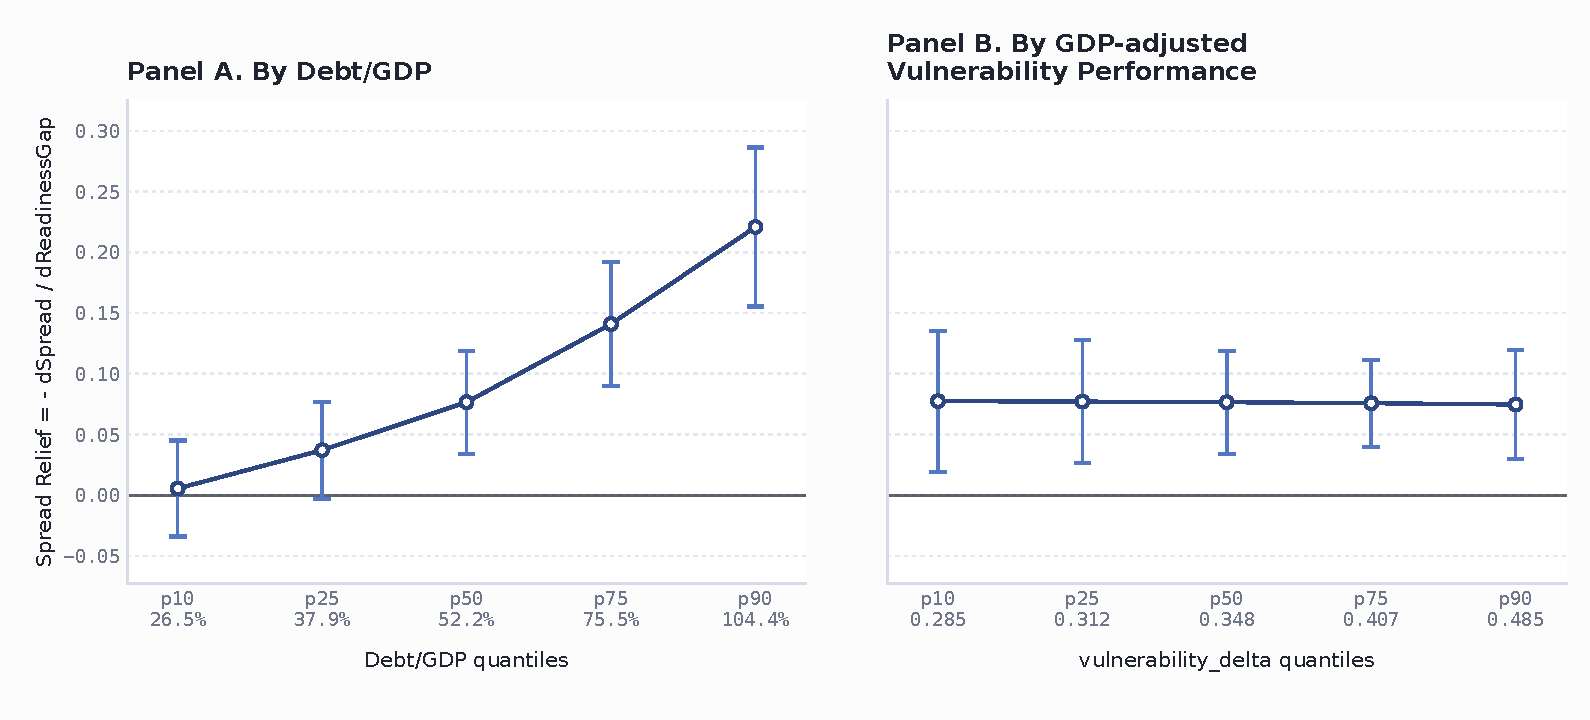
\includegraphics[width=\textwidth]{../appendixC/result/figure2.pdf}
\caption{Marginal Spread Relief from the Full-Interaction Spread Model, Level-Proxies}
\label{fig:appc_spread_relief}
\begin{minipage}{0.96\textwidth}
\footnotesize
\textit{Notes:} Panel A fixes $X_{it}$ at its median. Panel B fixes $B_{it}$ at its median. This appendix varies the level vulnerability proxy rather than the GDP-adjusted vulnerability-performance measure used in the main specification.
\end{minipage}
\end{figure}

Figure~\ref{fig:appc_theta_distribution} plots the country-year distribution of $\widehat\theta^F_{it}$ and country-level average rankings under the level-proxy construction. The dashed line marks the preferred empirical cutoff selected by the without-theta-controls kink specification.

\begin{figure}[H]\centering
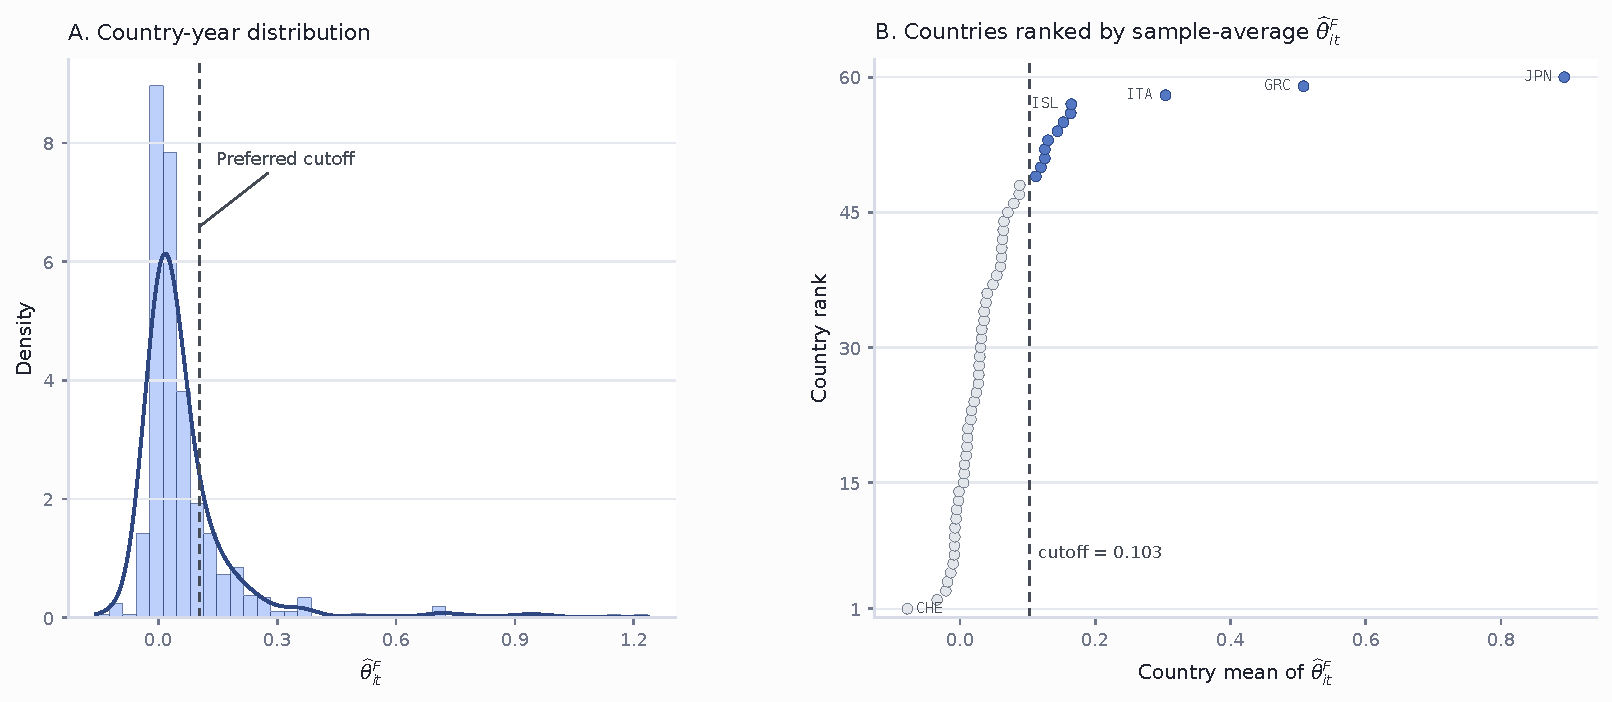
\includegraphics[width=\textwidth]{../appendixC/result/figure1_theta_distribution_cutoff.pdf}
\caption{Distribution of the Empirical Debt-Improving Index, Level-Proxies}
\label{fig:appc_theta_distribution}
\begin{minipage}{0.96\textwidth}
\footnotesize
\textit{Notes:} The left panel plots the country-year distribution of $\widehat\theta^F_{it}$. The right panel ranks countries by sample-average $\widehat\theta^F_{it}$. The dashed line marks the preferred empirical cutoff from the without-theta-controls kink specification.
\end{minipage}
\end{figure}

\subsection{Debt Dynamics and the Continuous Theta Interaction}

The debt-change regressions follow equations~\eqref{eq:emp_deltaB}--\eqref{eq:emp_debt_theta}, using the level-proxy version of $\widehat\theta^F_{it}$. Table~\ref{tab:appc_debt_change} shows that the continuous theta interaction remains negative and statistically significant. This implies that observations with higher empirical debt-improving capacity have a lower marginal effect of readiness on next-period debt changes.

\begin{table}[H]\centering
\begin{threeparttable}
\caption{Debt-Change Regressions, Level-Proxies}
\label{tab:appc_debt_change}
\scriptsize
\setlength{\tabcolsep}{3.0pt}
\begin{tabularx}{\textwidth}{lYYY}
\toprule
Dependent variable & \multicolumn{3}{c}{$\Delta B_{i,t+1}=B_{i,t+1}-B_{it}$} \\
\midrule
$G_{it}$ & -0.103*** & -0.082** & -0.090** \\
 & (-2.614) & (-2.074) & (-2.118) \\
$G_{it}\times\widehat\theta^F_{it}$ &  & -0.277*** & 0.033 \\
 &  & (-3.619) & (0.057) \\
$\widehat\theta^F_{it}$ &  &  & -0.187 \\
 &  &  & (-0.520) \\
Real GDP & 8.171*** & 4.694*** & 4.523*** \\
 & (5.412) & (3.205) & (2.914) \\
Real GDP growth & -0.326*** & -0.369*** & -0.391*** \\
 & (-3.610) & (-4.180) & (-3.854) \\
CPI inflation & -0.166** & -0.166** & -0.161** \\
 & (-1.976) & (-2.027) & (-2.095) \\
Overall balance/GDP & -0.468*** & -0.448*** & -0.436*** \\
 & (-5.849) & (-5.572) & (-5.160) \\
International reserves & 0.020 & -0.007 & -0.005 \\
 & (1.465) & (-0.475) & (-0.350) \\
Government effectiveness & -1.913** & -1.174 & -1.111 \\
 & (-2.020) & (-1.222) & (-1.134) \\
Regulatory quality & 1.921** & 0.331 & -0.029 \\
 & (2.155) & (0.358) & (-0.025) \\
Terms of trade & 0.044*** & 0.035** & 0.036** \\
 & (2.774) & (2.355) & (2.500) \\
\midrule
Theta main effect & No & No & Yes \\
Controls $\mathbf{Z}_{it}$ & Yes & Yes & Yes \\
Country FE & Yes & Yes & Yes \\
Year FE & Yes & Yes & Yes \\
Observations & 1,060 & 1,060 & 1,060 \\
Countries & 60 & 60 & 60 \\
Adjusted $R^2$ & 0.425 & 0.443 & 0.444 \\
\bottomrule
\end{tabularx}
\begin{tablenotes}[flushleft]\footnotesize
\item Notes: Columns 1--3 report the baseline model, the continuous theta interaction model, and the full-theta dynamics model, respectively. The full-theta dynamics specification includes $\widehat\theta^F_{it}$ as a direct control. Robust $t$-statistics are reported in parentheses. *** $p<0.01$, ** $p<0.05$, * $p<0.10$.
\end{tablenotes}
\end{threeparttable}
\end{table}

\subsection{Grouped Debt-Change Heterogeneity}

Table~\ref{tab:appc_grouped_debt_change} compares theta, debt-ratio, and marginal-relief sorts under the level-proxy construction. The theta and marginal-relief panels show more negative coefficients in higher groups, while the debt-ratio sort is less monotone. This is consistent with the interpretation that the composite index $B_{it}\widehat m^{G,F}_{it}$ captures more than debt exposure alone.

\begin{table}[H]\centering
\caption{Grouped Debt-Change Heterogeneity Regressions, Level-Proxies}
\label{tab:appc_grouped_debt_change}
\begin{threeparttable}
\scriptsize
\setlength{\tabcolsep}{3.0pt}
\renewcommand{\arraystretch}{1.10}
\textbf{Panel A. Full-theta groups}\\[0.45em]
\begin{tabularx}{\textwidth}{lYYYYY}
\toprule
Dependent variable & \multicolumn{5}{c}{$B_{i,t+1}-B_{it}$} \\
\cmidrule(lr){2-6}
Group & 0--20\% & 20--40\% & 40--60\% & 60--80\% & 80--100\% \\
\midrule
$G_{it}$ & 0.008 & -0.001 & -0.234*** & -0.133 & -0.417 \\
 & (0.045) & (-0.017) & (-2.803) & (-1.139) & (-1.622) \\
\midrule
Controls $\mathbf{Z}_{it}$ & Yes & Yes & Yes & Yes & Yes \\
Country FE & Yes & Yes & Yes & Yes & Yes \\
Year FE & Yes & Yes & Yes & Yes & Yes \\
Observations & 212 & 212 & 212 & 212 & 212 \\
Countries & 23 & 35 & 41 & 38 & 24 \\
Adjusted $R^2$ & 0.597 & 0.550 & 0.412 & 0.489 & 0.576 \\
\bottomrule
\end{tabularx}

\vspace{0.75em}
\textbf{Panel B. Debt-ratio groups}\\[0.45em]
\begin{tabularx}{\textwidth}{lYYYYY}
\toprule
Dependent variable & \multicolumn{5}{c}{$B_{i,t+1}-B_{it}$} \\
\cmidrule(lr){2-6}
Group & 0--20\% & 20--40\% & 40--60\% & 60--80\% & 80--100\% \\
\midrule
$G_{it}$ & 0.033 & -0.157 & -0.164** & -0.167 & -0.604** \\
 & (0.533) & (-1.169) & (-2.220) & (-1.328) & (-2.443) \\
\midrule
Controls $\mathbf{Z}_{it}$ & Yes & Yes & Yes & Yes & Yes \\
Country FE & Yes & Yes & Yes & Yes & Yes \\
Year FE & Yes & Yes & Yes & Yes & Yes \\
Observations & 212 & 212 & 212 & 212 & 212 \\
Countries & 28 & 35 & 41 & 32 & 22 \\
Adjusted $R^2$ & 0.465 & 0.482 & 0.705 & 0.397 & 0.629 \\
\bottomrule
\end{tabularx}

\vspace{0.75em}
\textbf{Panel C. Marginal-relief groups}\\[0.45em]
\begin{tabularx}{\textwidth}{lYYYYY}
\toprule
Dependent variable & \multicolumn{5}{c}{$B_{i,t+1}-B_{it}$} \\
\cmidrule(lr){2-6}
Group & 0--20\% & 20--40\% & 40--60\% & 60--80\% & 80--100\% \\
\midrule
$G_{it}$ & 0.037 & 0.045 & -0.161* & -0.316*** & -0.434 \\
 & (0.223) & (0.598) & (-1.821) & (-3.129) & (-1.426) \\
\midrule
Controls $\mathbf{Z}_{it}$ & Yes & Yes & Yes & Yes & Yes \\
Country FE & Yes & Yes & Yes & Yes & Yes \\
Year FE & Yes & Yes & Yes & Yes & Yes \\
Observations & 212 & 212 & 212 & 212 & 212 \\
Countries & 25 & 34 & 41 & 38 & 27 \\
Adjusted $R^2$ & 0.576 & 0.610 & 0.413 & 0.697 & 0.588 \\
\bottomrule
\end{tabularx}
\begin{tablenotes}[flushleft]\footnotesize
\item Notes: Each column estimates the next-period change in debt/GDP on the level readiness proxy, $G_{it}$, within the indicated subgroup. Macro control coefficients and subgroup cutoff values are omitted for compactness. Robust $t$-statistics are reported in parentheses. *** $p<0.01$, ** $p<0.05$, * $p<0.10$.
\end{tablenotes}
\end{threeparttable}
\end{table}

\subsection{Single-Crossing Kink Test}

The single-crossing specification again estimates whether the marginal effect of readiness on next-period debt changes crosses zero as a function of $\widehat\theta^F_{it}$. For a candidate cutoff $c$, the estimated without-theta-controls model is
\begin{equation}
\Delta B_{i,t+1}
=
\alpha_i+\tau_t
+aG_{it}(c-\widehat\theta^F_{it})_+
+bG_{it}(\widehat\theta^F_{it}-c)_+
+\boldsymbol{\Gamma}'\mathbf{Z}_{it}
+\varepsilon_{it}.
\label{eq:appc_kink}
\end{equation}
The implied marginal effect is
\begin{equation}
m(\theta;c)
=
a(c-\theta)_+
+
b(\theta-c)_+.
\label{eq:appc_kink_marginal}
\end{equation}

Table~\ref{tab:appc_kink_model} selects an empirical cutoff of $c=0.103037$ in the main without-theta-controls specification. Below the cutoff, the estimated marginal effect is positive; above the cutoff, it is negative. The sign pattern is therefore consistent with the single-crossing interpretation under the level-proxy construction.

\begin{table}[H]\centering
\begin{threeparttable}
\caption{Single-Crossing Kink Marginal-Effect Model, Level-Proxies}
\label{tab:appc_kink_model}
\scriptsize
\setlength{\tabcolsep}{3.0pt}
\begin{tabularx}{0.78\textwidth}{lY}
\toprule
Dependent variable & $B_{i,t+1}-B_{it}$ \\
\midrule
$G_{it}(c-\widehat\theta^F_{it})_+$ & 0.726*** \\
 & (3.667) \\
$G_{it}(\widehat\theta^F_{it}-c)_+$ & -0.225*** \\
 & (-2.890) \\
\midrule
Cutoff $c$ & 0.103 \\
RSS & 1.912 \\
Share below cutoff & 0.810 \\
Selection rule & RSS minimum; sign-consistent \\
Controls $\mathbf{Z}_{it}$ & Yes \\
Country FE & Yes \\
Year FE & Yes \\
Observations & 1,060 \\
Adjusted $R^2$ & 0.447 \\
\bottomrule
\end{tabularx}
\begin{tablenotes}[flushleft]\footnotesize
\item Notes: The exact RSS-selected cutoff is $c=0.1030368341448663$. The model includes country and year fixed effects and $\mathbf{Z}_{it}$ controls, but does not include direct theta controls. Robust $t$-statistics are reported in parentheses. *** $p<0.01$.
\end{tablenotes}
\end{threeparttable}
\end{table}

Figure~\ref{fig:appc_kink_marginal_effect} plots the continuous marginal-effect curve implied by equation~\eqref{eq:appc_kink_marginal}. The confidence band is computed by the delta method using the robust variance-covariance matrix of the two kink coefficients.

\begin{figure}[H]\centering
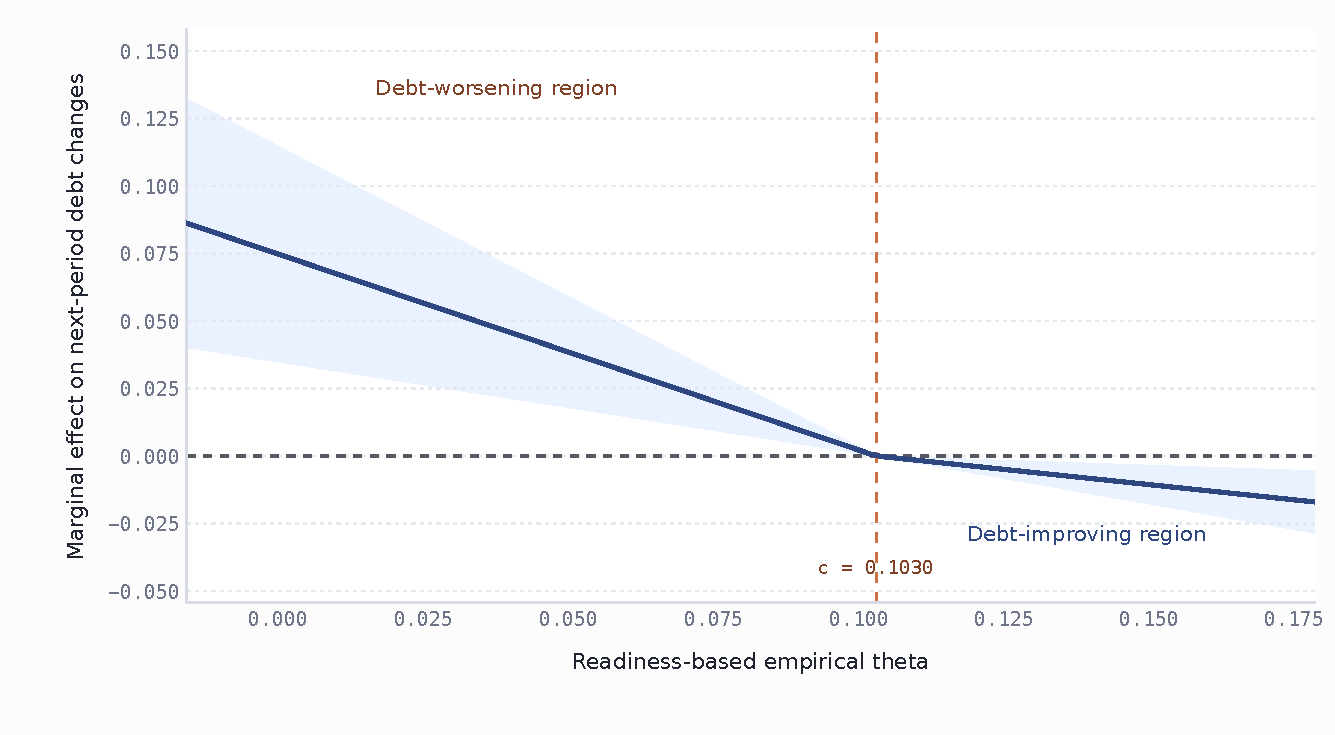
\includegraphics[width=0.92\textwidth]{../appendixC/result/figure3_kink_marginal_effect_notheta_continuous.pdf}
\caption{Continuous Kink Marginal Effect without Theta Controls, Level-Proxies}
\label{fig:appc_kink_marginal_effect}
\begin{minipage}{0.92\textwidth}
\footnotesize
\textit{Notes:} The figure plots $m(\theta;c)=a(c-\theta)_+ + b(\theta-c)_+$ from the single-crossing kink model without theta controls. Positive values imply that readiness improvements are associated with higher next-period debt changes; negative values imply lower next-period debt changes. The vertical dashed line marks the empirical cutoff $c$.
\end{minipage}
\end{figure}

\subsection{Country Screens Around the Preferred Cutoff}

Table~\ref{tab:appc_country_screens} applies the preferred cutoff to country-level screens. Under the level-proxy construction, no country satisfies the low-debt, always-above-cutoff, top-relief screening rule. Four countries satisfy the high-debt, always-below-cutoff, bottom-relief rule. As in the main text, the screen is descriptive and should not be interpreted as a structural country classification.

\begin{table}[H]\centering
\begin{threeparttable}
\caption{Country Screens Around the Preferred Cutoff, Level-Proxies}
\label{tab:appc_country_screens}
\scriptsize
\setlength{\tabcolsep}{3.0pt}
\textbf{Panel A. Low debt, theta always above the cutoff, and top-quartile marginal relief}\\[0.45em]
\begin{tabularx}{\textwidth}{llYYYYY}
\toprule
Country & ISO3 & Sample period & Years & Mean debt/GDP & Mean theta & Mean $\widehat m^{G,F}$ \\
\midrule
\multicolumn{7}{l}{No countries satisfy the screening rule.} \\
\bottomrule
\end{tabularx}

\vspace{0.75em}
\textbf{Panel B. High debt, theta always below the cutoff, and bottom-quartile marginal relief}\\[0.45em]
\begin{tabularx}{\textwidth}{llYYYYY}
\toprule
Country & ISO3 & Sample period & Years & Mean debt/GDP & Mean theta & Mean $\widehat m^{G,F}$ \\
\midrule
Croatia & HRV & 2008--2023 & 16 & 69.66\% & -0.021 & -0.034 \\
Malta & MLT & 2010--2023 & 14 & 53.91\% & -0.014 & -0.028 \\
Namibia & NAM & 2014--2023 & 10 & 53.74\% & -0.008 & -0.026 \\
Netherlands & NLD & 2000--2023 & 23 & 54.21\% & -0.007 & -0.016 \\
\bottomrule
\end{tabularx}
\begin{tablenotes}[flushleft]\footnotesize
\item Notes: The preferred cutoff is $c=0.103037$. Screening thresholds use country-level means: the mean-debt median is 53.06 percent, the bottom quartile of mean $\widehat m^{G,F}_{it}$ is 0.009, and the top quartile is 0.102. The always-above and always-below conditions are evaluated year by year.
\end{tablenotes}
\end{threeparttable}
\end{table}

\subsection{Additional Control-Set Variants}

This subsection reports the appendix control-set variants generated by the same workflow. The models parallel Appendix~\ref{appendixB}, but use the level readiness and vulnerability proxies throughout.

\begin{table}[H]\centering
\caption{Debt-Change Model Control-Set Variants, Level-Proxies}
\label{tab:appc_debt_change_control_variants}
\begin{threeparttable}
\scriptsize
\setlength{\tabcolsep}{3.0pt}
\renewcommand{\arraystretch}{1.02}
\textbf{Panel A. Baseline debt-change model}\\[0.45em]
\begin{tabularx}{\textwidth}{lYYY}
\toprule
Dependent variable & \multicolumn{3}{c}{$B_{i,t+1}-B_{it}$} \\
Control set & $\mathbf{Z}+B+X$ & $B+X$ & None \\
\midrule
$G_{it}$ & -0.066 & -0.125*** & -0.137*** \\
 & (-1.612) & (-2.898) & (-3.145) \\
$B_{it}$ & -0.085*** & -0.084*** &  \\
 & (-3.514) & (-3.951) &  \\
$X_{it}$ & 0.323 & -0.278 &  \\
 & (1.315) & (-1.276) &  \\
\midrule
Controls $\mathbf{Z}_{it}$ & Yes & No & No \\
Observations & 1,060 & 1,060 & 1,060 \\
Adjusted $R^2$ & 0.450 & 0.362 & 0.332 \\
\bottomrule
\end{tabularx}

\vspace{0.35em}
\textbf{Panel B. Continuous theta interaction model}\\[0.45em]
\begin{tabularx}{\textwidth}{lYYY}
\toprule
Dependent variable & \multicolumn{3}{c}{$B_{i,t+1}-B_{it}$} \\
Control set & $\mathbf{Z}+B+X$ & $B+X$ & None \\
\midrule
$G_{it}$ & -0.068* & -0.133*** & -0.139*** \\
 & (-1.664) & (-3.132) & (-3.289) \\
$G_{it}\times\widehat{\theta}^{F}_{it}$ & -0.100 & -0.232** & -0.332*** \\
 & (-0.905) & (-2.015) & (-4.858) \\
$B_{it}$ & -0.065* & -0.034 &  \\
 & (-1.808) & (-0.949) &  \\
$X_{it}$ & 0.343 & -0.142 &  \\
 & (1.399) & (-0.666) &  \\
\midrule
Controls $\mathbf{Z}_{it}$ & Yes & No & No \\
Observations & 1,060 & 1,060 & 1,060 \\
Adjusted $R^2$ & 0.450 & 0.369 & 0.368 \\
\bottomrule
\end{tabularx}

\vspace{0.35em}
\textbf{Panel C. Full-theta dynamics model}\\[0.45em]
\begin{tabularx}{\textwidth}{lYYY}
\toprule
Dependent variable & \multicolumn{3}{c}{$B_{i,t+1}-B_{it}$} \\
Control set & $\mathbf{Z}+B+X$ & $B+X$ & None \\
\midrule
$G_{it}$ & -0.069 & -0.141*** & -0.150*** \\
 & (-1.646) & (-2.979) & (-3.116) \\
$G_{it}\times\widehat{\theta}^{F}_{it}$ & -0.075 & -0.061 & -0.052 \\
 & (-0.131) & (-0.113) & (-0.095) \\
$\widehat{\theta}^{F}_{it}$ & -0.016 & -0.111 & -0.165 \\
 & (-0.047) & (-0.348) & (-0.507) \\
$B_{it}$ & -0.064** & -0.028 &  \\
 & (-2.199) & (-0.909) &  \\
$X_{it}$ & 0.339 & -0.160 &  \\
 & (1.260) & (-0.721) &  \\
\midrule
Controls $\mathbf{Z}_{it}$ & Yes & No & No \\
Observations & 1,060 & 1,060 & 1,060 \\
Adjusted $R^2$ & 0.450 & 0.368 & 0.368 \\
\bottomrule
\end{tabularx}
\begin{tablenotes}[flushleft]\footnotesize
\item Notes: Each specification includes country and year fixed effects. Robust $t$-statistics are reported in parentheses. *** $p<0.01$, ** $p<0.05$, * $p<0.10$.
\end{tablenotes}
\end{threeparttable}
\end{table}

For the $\mathbf{Z}_{it}+B_{it}+X_{it}$ version reported in Table~\ref{tab:appc_kink_notheta_controls}, the without-theta-controls kink specification is
\begin{equation}
\begin{aligned}
\Delta B_{i,t+1}
&=
\alpha_i+\tau_t
+aG_{it}(c-\widehat\theta^F_{it})_+
+bG_{it}(\widehat\theta^F_{it}-c)_+ \\
&\quad
+\delta_B B_{it}
+\delta_X X_{it}
+\boldsymbol{\Gamma}'\mathbf{Z}_{it}
+\varepsilon_{it}.
\end{aligned}
\label{eq:appc_kink_notheta_zbx}
\end{equation}

\begin{table}[H]\centering
\caption{Single-Crossing Kink without Theta Controls: Control-Set Variants, Level-Proxies}
\label{tab:appc_kink_notheta_controls}
\begin{threeparttable}
\scriptsize
\setlength{\tabcolsep}{3.0pt}
\begin{tabularx}{0.92\textwidth}{lYYY}
\toprule
Dependent variable & \multicolumn{3}{c}{$B_{i,t+1}-B_{it}$} \\
Control set & $\mathbf{Z}+B+X$ & $B+X$ & None \\
\midrule
$G_{it}(c-\widehat\theta^F_{it})_+$ & 1.078* & -0.202 & 0.141 \\
$p(a>0)$ & 0.050 & 0.783 & 0.240 \\
$G_{it}(\widehat\theta^F_{it}-c)_+$ & -0.118 & -0.188 & -0.339*** \\
$p(b<0)$ & 0.147 & 0.050 & 0.000 \\
\midrule
RSS cutoff & -0.002 & 0.042 & -0.016 \\
Sign-consistent & Yes & No & Yes \\
Country FE & Yes & Yes & Yes \\
Year FE & Yes & Yes & Yes \\
Observations & 1,060 & 1,060 & 1,060 \\
Adjusted $R^2$ & 0.451 & 0.366 & 0.364 \\
\bottomrule
\end{tabularx}
\begin{tablenotes}[flushleft]\footnotesize
\item Notes: These variants keep the main without-theta-controls kink structure but vary the additional controls. Reported $p$-values are one-sided tests for the sign restriction. *** $p<0.01$, * $p<0.10$.
\end{tablenotes}
\end{threeparttable}
\end{table}

For the $\mathbf{Z}_{it}+B_{it}+X_{it}$ version corresponding to Table~\ref{tab:appc_kink_withtheta_main}, the kink specification with direct theta controls is
\begin{equation}
\begin{aligned}
\Delta B_{i,t+1}
&=
\alpha_i+\tau_t
+aG_{it}(c-\widehat\theta^F_{it})_+
+bG_{it}(\widehat\theta^F_{it}-c)_+ \\
&\quad
+\rho_1\widehat\theta^F_{it}
+\rho_2(\widehat\theta^F_{it}-c)_+
+\delta_B B_{it}
+\delta_X X_{it}
+\boldsymbol{\Gamma}'\mathbf{Z}_{it}
+\varepsilon_{it}.
\end{aligned}
\label{eq:appc_kink_withtheta_zbx_main}
\end{equation}

\begin{table}[H]\centering
\begin{threeparttable}
\caption{Single-Crossing Kink with Theta Controls, Level-Proxies}
\label{tab:appc_kink_withtheta_main}
\scriptsize
\setlength{\tabcolsep}{3.0pt}
\begin{tabularx}{0.78\textwidth}{lY}
\toprule
Dependent variable & $B_{i,t+1}-B_{it}$ \\
\midrule
$G_{it}(c-\widehat\theta^F_{it})_+$ & 0.093 \\
 & (0.251) \\
$G_{it}(\widehat\theta^F_{it}-c)_+$ & 0.470 \\
 & (0.745) \\
\midrule
Direct theta controls & Yes \\
Cutoff $c$ & 0.179 \\
RSS & 1.896 \\
Share below cutoff & 0.900 \\
Selection rule & RSS minimum \\
Controls $\mathbf{Z}_{it}$ & Yes \\
Country FE & Yes \\
Year FE & Yes \\
Observations & 1,060 \\
Adjusted $R^2$ & 0.450 \\
\bottomrule
\end{tabularx}
\begin{tablenotes}[flushleft]\footnotesize
\item Notes: This appendix version includes $\widehat{\theta}^{F}_{it}$ and $(\widehat{\theta}^{F}_{it}-c)_+$ as direct controls. The with-theta-controls version does not satisfy the single-crossing sign pattern at the RSS-minimizing cutoff. Robust $t$-statistics are reported in parentheses.
\end{tablenotes}
\end{threeparttable}
\end{table}

For the $\mathbf{Z}_{it}+B_{it}+X_{it}$ column reported in Table~\ref{tab:appc_kink_withtheta_controls}, the estimated with-theta-controls variant uses the same control-augmented kink equation in \eqref{eq:appc_kink_withtheta_zbx_main}.

\begin{table}[H]\centering
\caption{Single-Crossing Kink with Theta Controls: Control-Set Variants, Level-Proxies}
\label{tab:appc_kink_withtheta_controls}
\begin{threeparttable}
\scriptsize
\setlength{\tabcolsep}{3.0pt}
\begin{tabularx}{0.92\textwidth}{lYYY}
\toprule
Dependent variable & \multicolumn{3}{c}{$B_{i,t+1}-B_{it}$} \\
Control set & $\mathbf{Z}+B+X$ & $B+X$ & None \\
\midrule
$G_{it}(c-\widehat\theta^F_{it})_+$ & 1.614** & 2.007*** & 1.495** \\
$p(a>0)$ & 0.020 & 0.004 & 0.018 \\
$G_{it}(\widehat\theta^F_{it}-c)_+$ & 0.141 & 0.234 & 0.232 \\
$p(b<0)$ & 0.593 & 0.660 & 0.656 \\
\midrule
RSS cutoff & 0.044 & 0.044 & 0.046 \\
Sign-consistent & No & No & No \\
Direct theta controls & Yes & Yes & Yes \\
Country FE & Yes & Yes & Yes \\
Year FE & Yes & Yes & Yes \\
Observations & 1,060 & 1,060 & 1,060 \\
Adjusted $R^2$ & 0.454 & 0.373 & 0.367 \\
\bottomrule
\end{tabularx}
\begin{tablenotes}[flushleft]\footnotesize
\item Notes: These variants keep direct theta controls and vary the additional controls across $\mathbf{Z}_{it}+B_{it}+X_{it}$, $B_{it}+X_{it}$, and no controls. Reported $p$-values are one-sided tests for the sign restriction. *** $p<0.01$, ** $p<0.05$.
\end{tablenotes}
\end{threeparttable}
\end{table}


\end{document}
